
% $Id: manual_tex.tex,v 1.2 2006-10-30 20:40:21 sarich Exp $ 
%
% LATEX version of the TAO users manual.
%
% manual_tex.tex is the base file for LaTeX format, while manual.tex is
% the corresponding base HTML format file.
%
% \documentclass[11pt]{../sty/report_tao}
\documentclass[dvipdfm,11pt,openright]{book}
%\usepackage[dvips]{graphicx}
\usepackage{epsf}
\usepackage{amssymb}
% moreverb provides commands for reading and writing files. In particular,
% verbatiminput. See pages 66-70 on the LateX Companion.
\usepackage{moreverb}
% float supersedes the obsolete here package. See page 149 of the LateX Companion.
\usepackage{float}
% url is a form of \verb intended for addresses, hypertext links, directories/paths,...
\usepackage{url}
\usepackage[bookmarksopen,colorlinks]{hyperref}
% afterpage places documents at the top of the page. See page 150 of the LateX Companion.
\usepackage{afterpage}

\setlength{\textwidth}{6.0in}
\setlength{\oddsidemargin}{18pt}
\setlength{\evensidemargin}{18pt}
\setlength{\topmargin}{-0.5in}
\setlength{\textheight}{8.5in}

\newcommand{\half}{{\textstyle{\frac{1}{2}}}}
%\newcommand{\findex}[1]{\index{FUNCTION #1}}
\newcommand{\findex}[1]{\index{#1}}
\newcommand{\sindex}[1]{\index{#1}}
\newcommand{\F}{\mbox{\boldmath \(F\)}}
\newcommand{\x}{\mbox{\boldmath \(x\)}}
\newcommand{\rr}{\mbox{\boldmath \(r\)}}
\newcommand{\R}{\mathbb R}
\renewcommand{\Re}{\R}
\newcommand{\Comment}[1]{}

\makeindex
 
% Defines the environment where design issues are discussed. In the manual
% version of this report, these regions are ignored.
\def\design{\medskip \noindent Design Issue:\begin{em}}
\def\enddesign{\end{em} \medskip}
% Manual version:
% \def\design{\comment}
% \def\enddesign{\endcomment}

% Print DRAFT in large letters across every page
%\special{!userdict begin /bop-hook{gsave 200 70 translate
%65 rotate /Times-Roman findfont 216 scalefont setfont
%0 0 moveto 0.95 setgray (DRAFT) show grestore}def end}

% Defines that we're doing the whole manual, not the short intro part,
% used in part1.tex.
\def\shortintro{false}

\begin{document}

\pagestyle {empty}

\vspace{1.75in}

\begin{center}

ARGONNE NATIONAL LABORATORY

9700 South Cass Avenue

Argonne, Illinois  60439

\vspace{1.5in}

{\Large
{\bf 
TAO Users Manual
}
}

\vspace{.5in}

{\bf Lois Curfman McInnes \\ Jorge J. Mor\'e \\ Todd Munson \\ Jason Sarich}

\vspace{.5in}

Mathematics and Computer Science Division

\vspace{.25in}

Technical Report  ANL/MCS-TM-242-Revision 1.10.1

\vspace{.25in}

This manual is intended for use with TAO version 1.10.1

\vspace{1.0in}

\today
\end{center}

\vspace{1.5in}

\par\noindent
This work was supported by the Mathematical, Information,
and Computational Sciences Division subprogram of the
Office of Computational and Technology Research,
U.S. Department of Energy, under Contract W-31-109-Eng-38.



% Table of contents.
\cleardoublepage
\pagestyle {plain}
\pagenumbering{roman}
\setcounter{page}{1}
\tableofcontents

% Abstract for users manual
\cleardoublepage
%\addcontentsline{toc}{chapter}{Preface}
% Abstract for TAO Users Manual

\section*{Preface}

The Toolkit for Advanced Optimization (TAO) focuses on the development
of algorithms and software for the solution of large-scale
optimization problems on high-performance architectures.  Areas of
interest include nonlinear least squares, unconstrained and
bound-constrained optimization, and general nonlinear optimization.

The development of TAO was motivated by the scattered support for
parallel computations and the lack of reuse of external toolkits in
current optimization software.  Our aim is to use object-oriented
techniques to produce high-quality optimization software for a range
of computing environments ranging from serial workstations and laptops
to massively parallel high-performance architectures.  Our design
decisions are strongly motivated by the challenges inherent in the use
of large-scale distributed memory architectures and the reality of
working with large, often poorly structured legacy codes for specific
applications.

This manual describes the use of TAO.
Since TAO is still under development, changes in usage and
calling sequences may occur.  TAO is fully supported; see the
the web site \url{http://www.mcs.anl.gov/tao} for information on
contacting the TAO developers.


%%% Local Variables: 
%%% mode: latex
%%% TeX-master: "manual_tex"
%%% End: 



% Acknowledgements for users manual
%\addcontentsline{toc}{chapter}{Acknowledgments}
% Acknowledgements for TAO Users Manual
%
% These are also listed on the TAO homepage, so if you add something here
% add it to the home page also
%

\section*{Acknowledgments}

The initial development of TAO was funded by the ACTS Toolkit Project in
the Office of Advanced Scientific Computing Research, U.S. Department
of Energy. We gratefully acknowledge their support.

TAO owes much to the developers of PETSc. We have benefitted
from their experience, tools, software, and advice. In many ways, TAO is a 
natural outcome of the PETSc development.
%
TAO has also benefitted from the work of various researchers
who have provided solvers, test problems, and interfaces.
In particular, we acknowledge

\begin{itemize}
\setlength{\itemsep}{0pt}
\item 
Lisa Grignon for contributing the least squares examples
\texttt{chebyq.c}, \texttt{coating.c}  and \texttt{enzreac1.c};
\item Yurii Zinchenko and Mike Gertz for the interface to
the OOQP solver for quadratic problems with linear constraints;
\item
Liz Dolan for developing the HTML version of the TAO user guide
\item
Boyana Norris for developing prototype CCA-compliant 
optimization component interfaces.
\item Gabriel Lopez-Calva for integrating ADIC with TAO on Distributed
Array applications and developing examples that use them; and
\item Jarek Nieplocha, Limin Zhang, and Manojkumar Krishnan for the
interface between Global Arrays and TAO and implemented example
applications.
\end{itemize}

\noindent
Finally, we thank all TAO users for their comments, bug reports, and
encouragement.

%%% Local Variables: 
%%% mode: latex
%%% TeX-master: "manual_tex"
%%% End: 


% Start of the Users Manual
\cleardoublepage
\setcounter {page}{1}
\pagenumbering{arabic}

\chapter{Introduction to TAO}
\label{chapter:introduction}

% Very introductory, gentle introduction. Pretty tables and figures.
% Perhaps use preamble of \ref{chapter:Getting Started}
% Written in C, but good with C++ compilers.  Also can use fortran.

The Toolkit for Advanced Optimization (TAO) focuses on the design and
implementation of optimization software for the
solution of large-scale optimization applications on high-performance
architectures.  Our approach is motivated by the scattered support for
parallel computations and lack of reuse of linear algebra software in
currently available optimization software.  The TAO design allows the
reuse of toolkits that provide lower-level support (parallel sparse
matrix data structures, preconditioners, solvers), and thus we are
able to build on top of these toolkits instead of having to redevelop
code. The advantages in terms of efficiency and development time are
significant.

The TAO design philosophy uses object-oriented techniques of data and
state encapsulation, abstract classes, and limited inheritance to
create a flexible optimization toolkit.  This chapter provides a short
introduction to our design philosophy by describing the objects in TAO
and the importance of this design.  Since a major concern in the TAO
project is the performance and scalability of optimization algorithms
on large problems, we also present some performance resuls.

\begin{comment}   

The Toolkit for Advanced Optimization (TAO) focuses on the design of large
scale optimization software, including nonlinear least
squares, unconstrained minimization, bound constrained
optimization, and decomposition techniques.
The solution of such problems
pervades many areas of computational science and demands robust and
flexible solution strategies.
As surveyed by Mor\'e and Wright \cite{optguide93},
various software packages are available for solving these
problems; however, their portability, versatility, and scalability are
restricted, especially within parallel environments.

The current generation of numerical software generally has a rigid form
that imposes many limitations, even when restricted to
uniprocessor architectures.
In traditional software design, the expressions of
algorithms make assumptions about the way mathematical objects, such as
vectors and matrices, are represented by the computer.
Thus, users are
forced to convert from the natural representation of data for a particular
application to one imposed by the software developer, often at the
expense of considerable overhead.  In addition, library routines are
often characterized by long and complicated calling sequences, with
no consistent interface among algorithms that solve a particular class
of problems.

These issues are magnified by the very nature of multiprocessor
architectures, since robust and
efficient implementation of mathematical abstractions involves
the added considerations
of parallel data structures and communication.
An effective software package should
exploit different parallel programming
techniques for various phases of the solution process.

Since many application problems require the computational
power of high-performance computers, a need clearly exists for a
uniform and flexible framework for developing optimization software and
solving application programs.
Our goal is to use object-oriented and component-based
software engineering techniques to create such an environment.

\end{comment}

\section{TAO Design Philosophy} 

%Use MPI, Microkernal 
% Goals, Current state of art. AD support
%\section{} Use matrices, vectors, linear solvers, as TAO objects

The TAO design philosophy place strongs emphasis on the reuse of
external tools where appropriate.  Our design enables bidirectional
connection to lower-level linear algebra support (e.g. parallel sparse
matrix data structures) provided in toolkits such as PETSc
\cite{petsc} \cite{petsc-user-ref,petsc-web-page}
as well as higher-level application
frameworks.  Our design decisions are strongly motivated by the
challenges inherent in the use of large-scale distributed memory
architectures and the reality of working with large and often poorly
structured legacy codes for specific applications.  Figure
\ref{tao:design} illustrates how the TAO software works with external
libraries and application code.

%\begin{figure}[ht]
%\centering{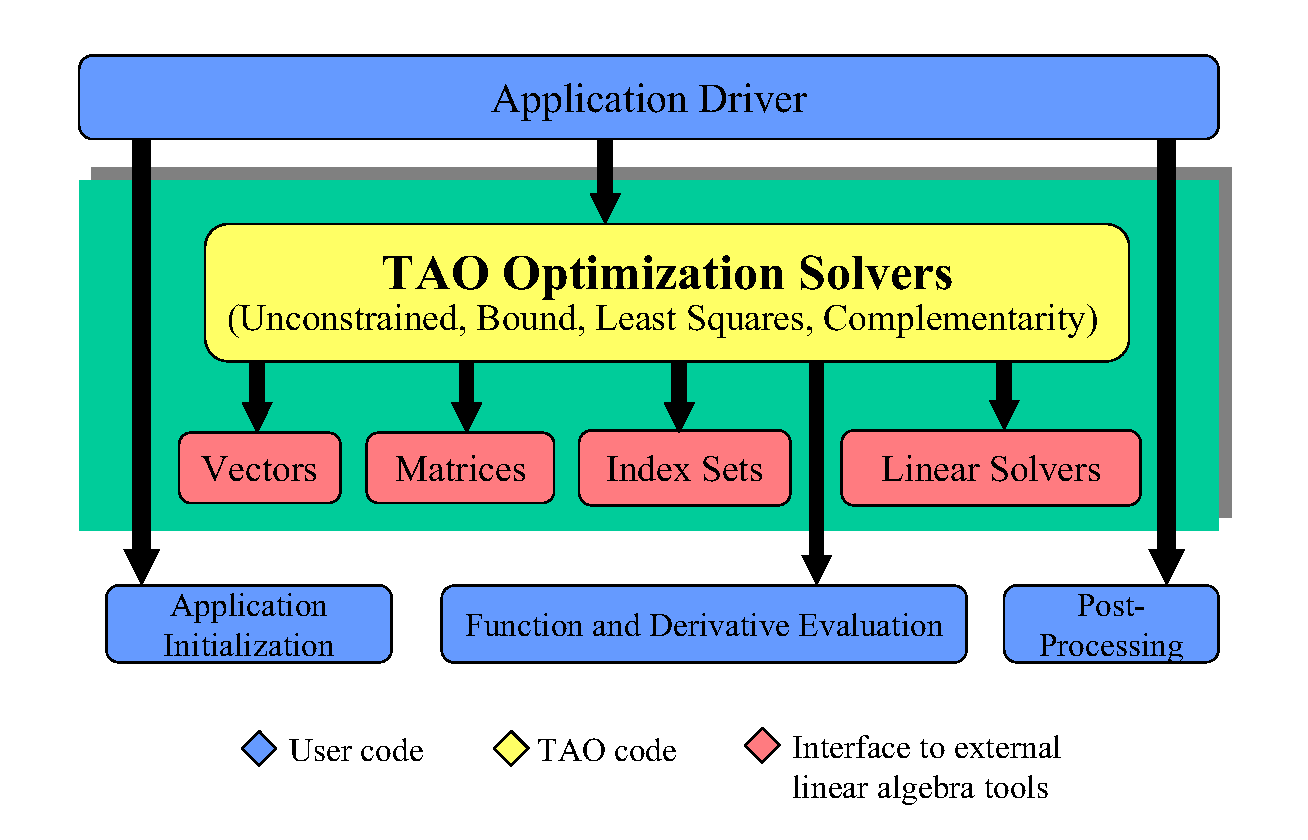
\includegraphics[height=3.5in,clip]{taofig.eps}}
%\caption{TAO Design}
%\label{tao:design}
%\end{figure}

\begin{figure}
\centerline{\epsfysize=3.5in \epsfbox{taofig.eps}}
\caption{TAO Design}
\label{tao:design}
\end{figure}


The TAO solvers use four fundamental objects to define and solve
optimization problems: vectors, index sets, matrices, and linear
solvers.  The concepts of vectors and matrices are standard, while an
index set refers to a set of integers used to identify particular
elements of vectors or matrices.  An optimization algorithm is a
sequence of well defined operations on these objects.  These
operations include vector sums, inner products, and matrix-vector
multiplication.  TAO makes no assumptions about the representation of
these objects by passing pointers to data-structure-neutral objects
for the execution of these numerical operations.

With sufficiently flexible abstract interfaces, TAO can support a
variety of implementations of data structures and algorithms.  These
abstractions allow us to more easily experiment with a range of
algorithmic and data structure options for realistic problems, such as
within this case study.  Such capabilities are critical for making
high-performance optimization software adaptable to the continual
evolution of parallel and distributed architectures and the research
community's discovery of new algorithms that exploit their features.

Our current TAO implementation uses the parallel system
infrastructure and linear algebra objects offered by PETSc,
which uses MPI \cite{using-mpi} for all interprocessor communication.
The PETSc package supports objects for vectors, matrices, index 
sets, and linear solvers.

The TAO design philosophy eliminates some of the barriers in using
independently developed software components by accepting data that is
independent of representation and calling sequence written for
particular data formats.  The user can initialize an application with
external frameworks, provide function information to a TAO solver, and
call TAO to solve the application problem.

The use of abstractions for matrices and vectors in TAO optimization
software also enables us to leverage automatic differentiation
technology to facilitate the parallel computation of gradients and
Hessians needed within optimization algorithms.  We have demonstrated
the viability of this approach through preliminary interfacing between
TAO solvers and the automatic differentiation tools ADIFOR and ADIC.
We are currently working on developing TAO interfaces that use special
problem features (for example, partial separability, stencil
information) in automatic differentiation computations.

\section{Performance Results}

A major concern in the TAO project is the performance and scalability
of optimization algorithms on large problems.  In this section we
focus on the GPCG (gradient projection, conjugate gradient) algorithm
for the solution of bound-constrained convex quadratic programming
problems.  Originally developed by Mor\'e and Toraldo
\cite{more-toraldo}, the GPCG algorithm was designed for large-scale
problems but had only been implemented for a single processor.  GPCG
combines the advantages of the identification properties of the
gradient projection method with the finite termination properties of
the conjugate gradient method.  Moreover, the performance of the
TAO implementation on large optimization problems is noteworthy.

%\begin{figure}[tb]
%\centering{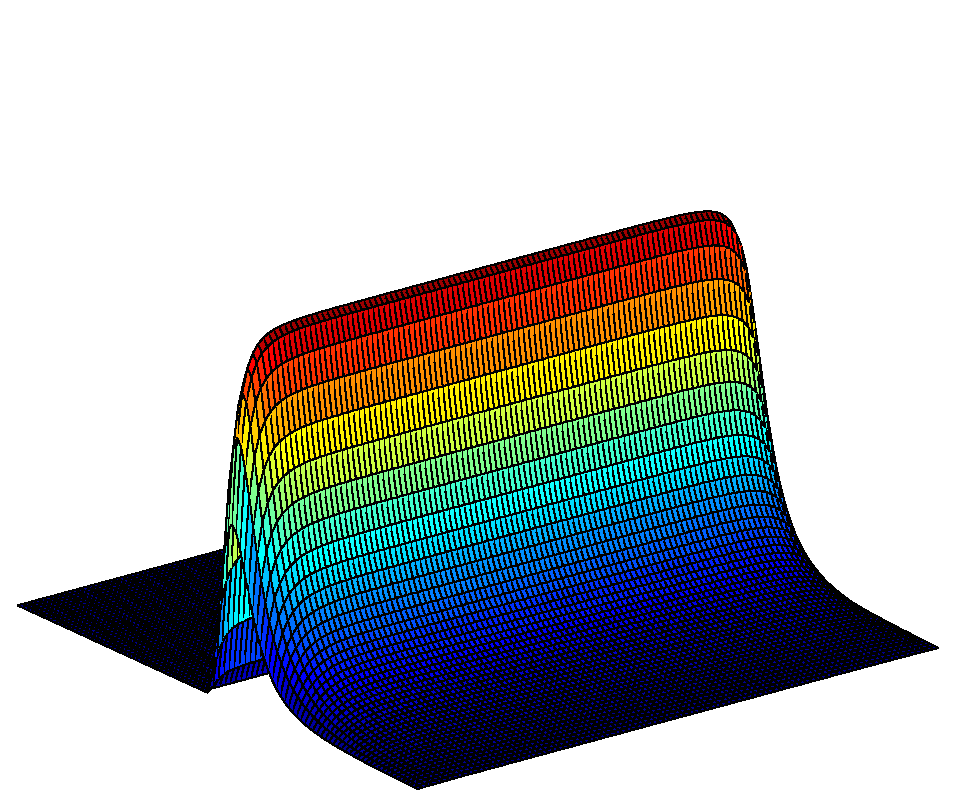
\includegraphics[height=3.0in]{pjb.eps}}
%\caption{The journal bearing problem with $\epsilon$ = 0.9}
%\label{dpjb}
%\end{figure}

\begin{figure}[tb]
\centerline{\epsfysize=3.0in \epsfbox{pjb.eps}}
\caption{The journal bearing problem with $\epsilon$ = 0.9}
\label{dpjb}
\end{figure}



We illustrate the performance of the GPCG algorithm by 
presenting results for a journal bearing problem
with over 2.5 million variables.
The journal bearing problem
is a finite element approximation to a variational problem 
over a rectangular two-dimensional grid.  A
grid with $1600$ points in each direction, for example, is formulated
as a bound constrained quadratic problem with $1600^2=2,560,000$
variables.
The triangulation of the grid results in a matrix that has the
usual five diagonal nonzero structure that arises
from a difference approximation to the Laplacian operator.
The journal bearing problem contains an eccentricity parameter,
$\varepsilon \in (0,1)$, that influences the number of active
variables at the solution and the difficulty in solving it.
Figure \ref{dpjb} shows the solution of the journal bearing problem
for $ \varepsilon = 0.9 $. The steep gradient in the solution
makes this problem a difficult benchmark.

The performance results in Table \ref{flops} are noteworthy is several
ways.  First of all, the number of faces visited by GPCG is remarkably
small.  Other strategies can lead to a large number of gradient
projection iterates, but the GPCG algorithm is remarkably efficient.
Another interesting aspect of these results is that due to the low
memory requirements of iterative solvers, we were able to solve these
problems with only $ p = 8 $ processors.  Strategies that rely on
direct solvers are likely to need significantly more storage, and thus
more processors.  Finally, these results show that the GPCG
implementation has excellent efficiency.  For example, the efficiency
of GPCG with respect to $ p = 8 $ processors ranges between $ 70\% $
and $ 100\% $ when $ \varepsilon = 0.1 $.  This sustained efficiency
is remarkable since the GPCG algorithm is solving a sequence of linear
problems with a coefficient matrix set to the submatrix of the Hessian
matrix with respect to the free variables for the current iterate.
Thus, our implementation's repartitioning of submatrices effectively
deals with the load-balancing problem that is inherent in the GPCG
algorithm.

\begin{table}[htb]
\begin{center}
\begin{tabular}{| c r | c c r c r |}
\hline
\multicolumn{1}{|c}{$ \varepsilon $} & 
\multicolumn{1}{c|}{$ p $} & 
\multicolumn{1}{c}{faces} &
\multicolumn{1}{c}{$n_{CG}$} & 
\multicolumn{1}{c}{time} &
\multicolumn{1}{c}{$t_{CG}$\%} & 
\multicolumn{1}{c|}{$ \cal E $} \\ \hline
0.1  & 8 & 46 & 431 & 7419 & 86 & 100  \\ 
0.1  & 16 & 45 & 423 & 3706 & 83 & 100  \\
0.1  & 32 & 45 & 427 & 2045 & 82 & 91 \\
0.1  & 64 & 45 & 427 & 1279 & 82 & 73 \\
\hline
0.9  & 8 & 37 & 105 & 2134 & 70 & 100 \\
0.9  & 16 & 37 & 103 & 1124 & 71 & 95 \\
0.9  & 32 & 38 & 100 & 618 & 69 & 86 \\
0.9  & 64 & 38 & 99 & 397 & 68 & 67 \\
\hline
\end{tabular}
\caption{Performance of GPCG on the journal bearing problem
with $ 2.56 \cdot 10^6 $ variables.}
\label{flops}
\end{center}
\end{table}




An important aspect of our results that is not
apparent from Table \ref{flops} is that 
for these results we were able to experiment easily 
with all the preconditioners offered by PETSc.
In particular, we were able to compare the diagonal Jacobi
preconditioner with block Jacobi and overlapping additive Schwarz
preconditioners that use a zero-fill ILU solver in each block.  We
also experimented with a parallel zero-fill incomplete Cholesky preconditioner
provided by a PETSc interface to the BlockSolve95~\cite{bs-user-ref}
package of Jones and
Plassmann.  Interestingly enough, the diagonal Jacobi preconditioner
achieved better performance on this problem.



%%% Local Variables: 
%%% mode: latex
%%% TeX-master: "manual_tex"
%%% End: 


\chapter{Getting Started}
\label{chapter:intro_tao}

TAO can be used on a personal
computer with a single processor or within a parallel environment.  
Its basic usage involves only a few commands, but fully 
understanding its usage requires time.
Application programmers can easily begin to use TAO by working with 
some examples provides in the package
and then gradually learn more details according to
their needs.  The current version of TAO and the most recent help 
concerning the installation and usage of TAO can be found at  
\url{http://www.mcs.anl.gov/tao/}.

The current version (1.10.1) of TAO requires an ANSI C++ compiler, 
an implementation of MPI, Version 3.1 of PETSc compiled with the C++ 
compiler, (PETSc must be configured with the \texttt{--with-clanguage=C++}
option) and at 
least 15 MB of free disk space.
During the setup process, the user will have to set an environmental
variable, \texttt{TAO\_DIR}\findex{TAO_DIR}, indicating the full path of 
the TAO home directory.
This variable will be used in this
manual to refer to the location of files, and by computers that
will compile TAO source code.

\section{Writing Application Codes with TAO}

The examples throughout the library demonstrate the software usage and
can serve as templates for developing custom applications.  We suggest
that new TAO users examine programs in
\begin{verbatim}
   ${TAO_DIR}/src/examples .
\end{verbatim} % Needed to fool the xemacs coloring algorithm $
\noindent
Additional examples are available on our website and in
\begin{verbatim}
   ${TAO_DIR}/src/<unconstrained,bound,..>/examples/tutorials,
\end{verbatim} 
% $
\noindent
where \texttt{<component>}
denotes any of the TAO components, such as 
\texttt{bound} or \texttt{unconstrained}.
The HTML version of the manual pages located at
\begin{verbatim}
   ${TAO_DIR}/docs/manualpages/index.html
\end{verbatim} % To fool the coloring algorithm $
\noindent
or
\begin{verbatim}
   http://www.mcs.anl.gov/tao/documentation/manualpages/index.html
\end{verbatim}
\noindent
provides indices (organized by both routine names and concepts) to the
tutorial examples.

We suggest the following procedure for writing a new application
program using TAO:

\begin{enumerate}
\item Install TAO according to the instructions in
  \url{http://www.mcs.anl.gov/tao/documentation/index.html}.
\item Copy the examples and makefile from the directory
  \url{${TAO\_DIR}/examples/}, compile the examples, and run the
  programs.
\item Select the example program matching the application most
  closely, and use it as a starting point for developing a customized
  code.
\end{enumerate}

\section{A Simple TAO Example}
\label{sec:simple}

To help the user start using TAO immediately, we use a simple
uniprocessor example. The code in
Figure~\ref{fig:example1} is for minimizing the
extended Rosenbrock function $f: \Re^n \to \Re$ defined by
\[
 f(x) = 
 \sum_{i=0}^{m-1} \left( \alpha(x_{2i+1}-x_{2i}^2)^2 + (1-x_{2i})^2 \right),
\]
where $n = 2m$ is the number of variables.  The code in
Figure~\ref{fig:example1} is only the main program.  We have not
included the code for evaluating the function and gradient or
for evaluating the Hessian matrix.

\afterpage{
\begin{figure}[H]
  {\footnotesize \verbatiminput{rosenbrock1.c}}
\caption{Example of Uniprocessor TAO Code\label{fig:example1}}
\end{figure}
}

Note that while we use the C language to introduce the TAO software,
the package is also fully usable from C++ and Fortran77/90.
Section~\ref{chapter:petscfapp} discusses additional issues concerning
Fortran usage.

The code in Figure~\ref{fig:example1} contains many of the components
needed to write most TAO programs and thus, is illustrative of the
features present in complex optimization problems.  Note that we have
omitted the code required for the routine \texttt{FormFunctionGradient},
which evaluates the function and gradient, and the code for
\texttt{FormHessian}, which evaluates the Hessian matrix for Rosenbrock's
function.  The following sections annotates the lines of code in
Figure~\ref{fig:example1}.

\section{Include Files}

The C++ include file for TAO should be used via the statement
\begin{verbatim}
   #include "tao.h"
\end{verbatim}
\noindent
The required lower level include files are automatically included
within this high-level file.

\section{TAO Initialization}
\label{sec:initialization}

All TAO programs contain a call to \findex{TaoInitialize()}
\begin{verbatim}
   info = TaoInitialize(int *argc,char ***argv,char *file_name, 
                        char *help_message);
\end{verbatim}
\noindent 
This command initializes TAO (and also MPI and PETSc if these have not
yet been initialized elsewhere).  The arguments \texttt{argc} and
\texttt{argv} are the command line arguments delivered in all C and
C++ programs. \sindex{command line arguments} The argument
\texttt{file\_name} optionally indicates an alternative name for an
options file, which by default is called \texttt{.petscrc} and resides
in the user's home directory.  See the PETSc users manual for details
regarding runtime option specification.  The final argument,
\texttt{help\_message}, is an optional character string that will be
printed if the program is run with the \texttt{-help} option.

As illustrated by the \texttt{TaoInitialize()} statement above, TAO
routines return an integer indicating whether an error has occurred
during the call.  The error code is set to be nonzero if an error has
been detected; otherwise, it is zero.  For the C or C++ interface, the
error variable is the routine's return value, while for the Fortran
version, each TAO routine has as its final argument an integer error
variable.  Error tracebacks are discussed in
Section~\ref{sec:tao_programming}.

\section{TAO Finalization}

All TAO programs should call \texttt{TaoFinalize()}
\findex{TaoFinalize()} as their final (or nearly final) statement
\findex{TaoFinalize()}
\begin{verbatim}
   info = TaoFinalize();
\end{verbatim}
\noindent
This routine handles options to be called at the conclusion of the
program, and calls \texttt{PetscFinalize()} %\findex{PetscFinalize()}
if \texttt{TaoInitialize()} began PETSc. If PETSc was initiated
externally from TAO (by either the user or another software package),
the user is responsible for calling \texttt{PetscFinalize()}.

\section{TAO Solvers}

The primary commands for solving an unconstrained optimization problem
using TAO are shown in Figure \ref{fig:tao_commands}.
\findex{TaoCreate()} \findex{TaoApplicationCreate()} \findex{TaoSetObjectiveAndGradientRoutine()}
\findex{TaoSetHessianMat()} \findex{TaoSolveApplication()}
\findex{TaoDestroy()} \findex{TaoSetInitialSolutionVec()}
\findex{TaoSetHessianRoutine()} \findex{TaoSolveApplication()} 
\findex{TaoApplicationDestroy()}

\begin{figure}[H]
\begin{verbatim}
   TaoCreate(MPI_Comm comm, TaoMethod method, TAO_SOLVER *tao); 
   TaoApplicationCreate(MPI_Comm comm, TAO_APPLICATION *taoapp); 
   TaoSetInitialSolutionVec(TAO_APPLICATION taoapp, Vec x);
   TaoSetObjectiveAndGradientRoutine(TAO_APPLICATION taoapp,
            int (*FormFGradient)(TAO_APPLICATION,Vec,double,Vec,void*),void *user);
   TaoSetHessianMat(TAO_APPLICATION taoapp, Mat H, Mat Hpre);
   TaoSetHessianRoutine(TAO_APPLICATION taoapp,
            int (*Hessian)(TAO_APPLICATION, Vec, Mat*, Mat*, MatStructure*, void*),(void *)&user);
   TaoSolveApplication(TAO_APPLICATION taoapp, TAO_SOLVER tao);
   TaoApplicationDestroy(TAO_APPLICATION taoapp);
   TaoDestroy(TAO_SOLVER tao);
\end{verbatim}
\caption{Commands for solving an unconstrained optimization problem
\label{fig:tao_commands}}
\end{figure}

\noindent
The user first creates the \texttt{TAO\_SOLVER} and
\texttt{TAO\_APPLICATION} contexts. He then sets call-back routines as
well as vector (\texttt{Vec}) and matrix (\texttt{Mat}) data
structures that the TAO solver will use for evaluating the
minimization function, gradient, and optionally the Hessian matrix.
The user then solves the minimization problem, and finally destroys
the \texttt{TAO\_SOLVER} and \texttt{TAO\_APPLICATION} contexts.
Details of these commands are presented in
Chapter~\ref{chapter:tao_solver}.

Note that \texttt{TaoCreate()} enables the user to select the solution
method at runtime by using an options database.  Through this
database, the user not only can select a minimization method (e.g.,
limited-memory variable metric, conjugate gradient, Newton with line
search or trust region), but also can prescribe the convergence
tolerance, set various monitoring routines, indicate techniques for
linear systems solves, etc.  See Chapter~\ref{chapter:tao_solver} for more 
information on the solver methods available in TAO.

\section{Function Evaluations}

Users of TAO are required to provide routines that perform function
evaluations. Depending on the solver chosen, they may also have to
write routines that evaluate the gradient vector and Hessian matrix.

\section{TAO Programming with PETSc}
\label{sec:tao_programming}

\subsection*{Include Files}

Applications using the PETSc package for vectors, matrices, and linear
solvers should include the appropriate header files.  For example
\begin{verbatim}
   #include "petscksp.h"
\end{verbatim}
\noindent
includes the appropriate information for most TAO applications using PETSc.

\subsection*{The Options Database}
\label{sec:options}

The user can input control data at run time using an options database.
The command
\begin{verbatim}
   PetscOptionsGetInt(PETSC_NULL, "-n", &user.n, &flg);
\end{verbatim}
\noindent
checks whether
the user has provided a command line option to set the value of \texttt{
n}, the number of variables.  If so, the variable \texttt{n} is set
accordingly; otherwise, \texttt{n} remains unchanged. A complete
description of the options database may be found in the PETSc users
manual.

\subsection*{Vectors}

In the example in Figure \ref{fig:example1}, the vector data structure
(\texttt{Vec}) is used to store the solution and gradient for TAO
unconstrained minimization solvers.  A new parallel or sequential
vector \texttt{x} of global dimension \texttt{M} is created with the
command % \findex{VecCreate()} \sindex{vectors}
\begin{verbatim}
   info = VecCreate(MPI_Comm comm,int m,int M,Vec *x);
\end{verbatim}
\noindent
where \texttt{comm} denotes the MPI communicator. The type of storage
for the vector may be set with either calls to \texttt{VecSetType()}
or \texttt{VecSetFromOptions()}.  Additional vectors of the same type
can be formed with % \findex{VecSetType()} \findex{VecSetFromOptions} \findex{VecDuplicate()}
\begin{verbatim}
   info = VecDuplicate(Vec old,Vec *new);
\end{verbatim}
\noindent
The commands % \findex{VecSet()} \findex{VecSetValues()}
\begin{verbatim}
   info = VecSet(Vec X,PetscScalar value);
   info = VecSetValues(Vec x,int n,int *indices,
                       Scalar *values,INSERT_VALUES);
\end{verbatim}
\noindent
respectively set all the components of a vector to a particular scalar
value and assign a different value to each component.  More detailed
information about PETSc vectors, including their basic operations,
scattering/gathering, index sets, and distributed arrays, may be found
in the PETSc users manual.

\subsection*{Matrices}

Usage of matrices and vectors is similar. \sindex{matrix} 
The user can create a new parallel or sequential matrix \texttt{H} with 
\texttt{M} global rows and \texttt{N} global columns, with the routine
%\findex{MatCreate()}
\begin{verbatim}
   info = MatCreate(MPI_Comm comm,int m,int n,int M,int N,Mat *H);
\end{verbatim}
\noindent
where the matrix format can be specified at runtime.  The user could
alternatively specify each processes' number of local rows and columns
using \texttt{m} and \texttt{n}.  \texttt{H} can then be used to store
the Hessian matrix, as indicated by the above routine
\texttt{TaoSetHessianMat()}.  Matrix entries can then be set with the
command
\begin{verbatim}
   info = MatSetValues(Mat H,int m,int *im,int n,int *in,
                       Scalar *values,INSERT_VALUES);
\end{verbatim}
\noindent
After %\findex{MatSetValues()} 
all elements have been inserted into the
matrix, it must be processed with the pair of commands
%\findex{MatAssemblyBegin()} \findex{MatAssemblyEnd()}
\begin{verbatim}
   info = MatAssemblyBegin(Mat H,MAT_FINAL_ASSEMBLY);
   info = MatAssemblyEnd(Mat H,MAT_FINAL_ASSEMBLY);
\end{verbatim}
\noindent
The PETSc users manual discusses various matrix formats as
well as the details of some basic matrix manipulation routines.

\subsection*{Parallel Programming}

Since TAO uses the message-passing model for parallel programming and
employs MPI for all interprocessor communication, the user is free to
employ MPI routines as needed throughout an application code.
However, by default the user is shielded from many of the details of
message passing within TAO, since these are hidden within parallel
objects, such as vectors, matrices, and solvers.  In addition, TAO
users can interface to external tools, such as the generalized vector
scatters/gathers and distributed arrays within PETSc, to assist in the
management of parallel data.

%\sindex{collective operations} 
The user must specify a communicator
upon creation of any TAO objects (such as a vector, matrix, or solver)
to indicate the processors over which the object is to be distributed.
For example, some commands for matrix, vector, and solver creation
are:
\begin{verbatim}
   info = MatCreate(MPI_Comm comm,int m,int n,int M,int N,Mat *H);
   info = VecCreate(MPI_Comm comm,int m,int M,Vec *x);
   info = TaoCreate(MPI_Comm comm,TaoMethod method,TAO_SOLVER *tao); 
\end{verbatim}
\noindent
The creation routines are collective over all processors in the
communicator; thus, all processors in the communicator {\em must} call
the creation routine.  In addition, if a sequence of collective
routines is being used, the routines {\em must} be called in the same
order on each processor.

\section{Compiling and Running TAO}
\label{sec:running}

Compilation of the TAO numerical libraries and TAO application codes
requires three environmental variables to be set.  These three
variables, \texttt{TAO\_DIR}, \texttt{PETSC\_ARCH}, and \texttt{PETSC\_DIR},
are discussed more fully in the TAO installation instructions.

TAO uses a portable makefile system provided by the
PETSc~\cite{petsc-web-page,petsc-user-ref} library, which is discussed
further in Section~\ref{sec:makefiles}.  The TAO library can be
compiled with the command
\begin{verbatim}
   make
\end{verbatim}
\noindent
from the \texttt{TAO\_DIR} directory.  

Running a TAO application on a single processor can be done in the
usual way by entering the name of the executable and any command line
options.  Running programs in parallel, however, requires use of the
MPI library.  All TAO programs use the MPI (Message Passing Interface)
standard for message-passing communication \cite{MPI-final}.  Thus, to
execute TAO programs, users must know the procedure for beginning MPI
jobs on their selected computer system(s).  For instance, when using
the MPICH implementation of MPI \cite{mpich-web-page} and many others,
the following command initiates a program that uses eight processors:
%\findex{mpirun} \sindex{running TAO programs} 
\begin{verbatim}
  mpirun -np 8 tao_program_name tao_options
\end{verbatim}

\begin{comment}
  Figure~\ref{fig:exrun} illustrates compiling and running a TAO
  program using MPICH.  Note that different sites may have slightly
  different library and compiler names.
\end{comment}

\begin{comment}
  Users who are experiencing difficulties linking TAO programs should
  refer to the troubleshooting guide via the TAO home page {\tt
    http://www.mcs.anl.gov/tao} or the source code given by the file
  \texttt{{TAO\_DIR}/docs/troubleshooting.html}.
\end{comment}

\begin{comment}
\begin{figure}[htb]
{\footnotesize
\begin{verbatim}
[ember] ex2 -tao_method tao_nls -tao_monitor
iter = 0, Function value: -0.330579, Residual: 0.728961
iter = 1, Function value: -0.427745, Residual: 3.64242e-07
iter = 2, Function value: -0.427745, Residual: 2.03244e-12

[ember] mpirun -np 2 ex2 -tao_method tao_nls -tao_monitor
iter = 0, Function value: -0.330579, Residual: 0.728961
iter = 1, Function value: -0.427745, Residual: 3.63647e-07
iter = 2, Function value: -0.427745, Residual: 2.18415e-12

\end{verbatim}
}
\nobreak
\caption{Running a TAO Program}
\label{fig:exrun}
\end{figure}
  
\end{comment}


\section{Error Checking}

All TAO commands begin with the \texttt{Tao} prefix and return an
integer indicating whether an error has occurred during the call.  The
error code equals zero after the successful completion of the routine
and is set to a nonzero value if an error has been detected.  The
macro \texttt{CHKERRQ(info)} checks the value of \texttt{info} and calls an
error handler upon error detection.  \texttt{CHKERRQ()} should be used in
all subroutines to enable a complete error traceback.

In Figure \ref{fig:traceback} we indicate a traceback generated by
error detection within a sample program. The error occurred on line
1007 of the file \texttt{\$\{TAO\_DIR\}/src/interface/tao.c} in the
routine \texttt{TaoSetUp()} and was caused by nonconforming local lengths
of the parallel gradient and solution vectors, which must be
identically partitioned.  The \texttt{TaoSetUp()} routine was called from
the \texttt{TaoSolveApplication()} routine, which was in turn called on line 229 of
the \texttt{main()} routine in the program \texttt{ex2.c}.  The PETSc users
manual provides further details regarding error checking, including
information about the Fortran interface.

\begin{figure}[htb]
{\footnotesize
\begin{verbatim}
[ember] mpirun -np 2 ex2 -tao_lmvm
[0]PETSC ERROR: TaoSetUp() line 1007 in src/interface/tao.c
[0]PETSC ERROR:   Nonconforming object sizes!
[0]PETSC ERROR:   Gradient and solution vectors must be identically partitioned!
[0]PETSC ERROR: TaoSolveApplication() line 1739 in src/interface/tao.c
[0]PETSC ERROR: main() line 229 in src/unconstrained/examples/tutorials/ex2.c
[0] MPI Abort by user Aborting program !
[0] Aborting program!
p0_911:  p4_error: : 1
bm_list_912:  p4_error: interrupt SIGINT: 2
\end{verbatim}
}
\caption{Example of Error Traceback}
\label{fig:traceback}
\end{figure}

\noindent
When running the debugging version of the TAO software (PETSc configured 
with the \texttt{--with-debugging} option), checking is performed for 
memory corruption
(writing outside of array bounds, etc). The macros \texttt{CHKMEMQ} and
\texttt{CHKMEMA} can be called anywhere in the code to check the current
status of the memory for corruption.  By putting several (or many) of
these macros into an application code, one can usually track
down the code segment where corruption has occurred.

\section{Makefiles}
\label{sec:makefiles}

To manage code portability across a wide variety of UNIX systems, TAO
uses a makefile system that is part of the PETSc software.  This
section briefly discusses makefile usage from the perspective of
application programmers; see the ``makefiles'' chapter of the PETSc
users manual for additional details.

\subsection*{Compiling TAO Programs}

To make a program named \texttt{rosenbrock1}, one may use the command
\begin{verbatim}
   make PETSC_ARCH=arch rosenbrock1
\end{verbatim}
\noindent
which compiles a debugging or optimized version of the example and
automatically link the appropriate libraries.  The architecture, {\tt
  arch}, is one of \texttt{solaris, rs6000, IRIX, hpux}, etc. Note that
when using command line options with make (as illustrated above), one
must {\em not} place spaces on either side of the ``='' signs.  The
variable \texttt{PETSC\_ARCH} can also be set as an
environmental variable.

\subsection*{Sample Makefiles}

\begin{figure}[tbh]
{\footnotesize
\begin{verbatim}   
       CFLAGS    = 
       FFLAGS    = 
       CPPFLAGS  =
       FPPFLAGS  =
       
       include ${TAO_DIR}/bmake/tao_common
   
       rosenbrock1: rosenbrock1.o tao_chkopts
            -${CLINKER} -o rosenbrock1 rosenbrock1.o ${TAO_LIB} ${PETSC_SNES_LIB}
            ${RM} rosenbrock1.o
\end{verbatim} 
% $
}
\caption{Sample TAO Makefile for a Single Program}
\label{fig:make1}
\end{figure}

Maintaining portable TAO makefiles is very simple.  Figure
\ref{fig:make1} presents a minimal makefile for maintaining a single
program that uses the TAO library.  The most important line in this
makefile is the line starting with \texttt{include}:
\begin{verbatim}
   include ${TAO_DIR}/bmake/tao_common
\end{verbatim} 
% $
\noindent
\findex{TAO_LIB} This line includes other makefiles that provide the
needed definitions and rules for the particular base software
installations (specified by \texttt{\$\{TAO\_DIR\}} and {\tt
  \$\{PETSC\_DIR\}}) and architecture (specified by {\tt
  \$\{PETSC\_ARCH\}}), which are typically set as environmental
variables prior to compiling TAO source or programs.  As listed in the
sample makefile, the appropriate \texttt{include} file is automatically
completely specified; the user should {\em not} alter this statement
within the makefile.

Note that the variable \texttt{\$\{TAO\_LIB\}} (as listed on the link
line in this makefile) specifies {\em all} of the various TAO and
supplementary libraries in the appropriate order for correct linking.


\begin{comment}
  The second sample makefile, given in Figure~\ref{fig:make2},
  controls the generation of several example programs.  Again, the
  most important line in this makefile is the \texttt{include} line that
  includes the files defining all of the macro variables.
\end{comment}

Some additional variables that can be used in the makefile are defined
as follows:
\begin{itemize}
\item \texttt{CFLAGS, FFLAGS} - user-specified additional options for the
  C++ compiler and fortran compiler.
\item \texttt{CPPFLAGS, FPPFLAGS} - user-specified additional flags
        for the C++ preprocessor and fortran preprocesor.
\item \texttt{CLINKER, FLINKER} - the C++ and Fortran linkers. 
\item \texttt{RM} - the remove command for deleting files.
\item \texttt{TAO\_LIB} - all of the base TAO libraries and required supplementary libraries.
             \findex{TAO_LIB}
\item \texttt{TAO\_FORTRAN\_LIB} - the TAO Fortran interface
             library. \findex{TAO_FORTRAN_LIB}
\item \texttt{PETSC\_FORTRAN\_LIB} - the PETSc Fortran interface
             library. 
\end{itemize}

\section{Directory Structure}

The home directory of TAO contains the following subdirectories:

\begin{itemize}
\item \texttt{docs} - All documentation for TAO. The files \texttt{tao\_manual.ps}
                   and \texttt{manual/manual.html} contain the users manual in
                   PDF and HTML formats, respectively. Includes
                   the subdirectory
 \subitem - \texttt{manualpages} (manual pages for individual TAO routines).
% \item \texttt{bin} - Utilities and short scripts for use with TAO, including
\item \texttt{bmake} - Base TAO makefile directory.  
\item \texttt{include} - All include files for TAO that are visible to the user.
\item \texttt{examples} - Example problems and makefile.
% \item \texttt{include/finclude}    - TAO include files for Fortran programmers using 
%                                   the .F suffix (recommended).
% \item \texttt{include/pinclude}    - Private TAO include files that should {\em not} 
%                                  be used by application programmers.
\item \texttt{src} - The source code for all TAO components, which
                  currently includes
 \begin{itemize}
 \item \texttt{unconstrained} - unconstrained minimization,
 \item \texttt{bound} - bound constrained minimization.
 \item \texttt{complementarity} - mixed complementarity solvers.
 \item \texttt{least\_squares} - nonlinear least squares,
% \item \texttt{constrained} - constrained minimization,
 \end{itemize}
\end{itemize}

\noindent
Each TAO source code component directory has the following subdirectories:
\begin{itemize}
\item  \texttt{examples} - Example programs for the component, including
  \begin{itemize}
  \item \texttt{tutorials} - Programs designed to teach users about TAO.  These
          codes can serve as templates for the design of custom applicatinos.
  \item \texttt{tests} - Programs designed for thorough testing of TAO.  As such,
          these codes are not intended for examination by users.
  \end{itemize}
\item  \texttt{interface} - The calling sequences for the abstract interface  
        to the component.
        Code here does not know about particular implementations.
\item  \texttt{impls} - Source code for one or more implementations.
\item  \texttt{utils} - Utility routines.  Source here may know about the 
          implementations, but ideally will not know about implementations
          for other components.
\end{itemize}

%%% Local Variables: 
%%% mode: latex
%%% TeX-master: "manual_tex"
%%% End: 


%
% NOTES:  
%  - Be sure to place captions BEFORE labels in figures and tables!
%    Otherwise, numbering will be incorrect.  For example, use the following:
%       \caption{TAO Info}
%       \label{fig:taoinfo}
%  - Use \break to indicate a line break (needed to prevent long strings in
%    \tt mode from running of the page)
%
% ---------------------------------------------------------------

\chapter{Basic Usage of TAO Solvers}
%\sindex{continuous optimization}
\label{chapter:tao_solver}

TAO contains unconstrained minimization, bound constrained minimization, 
%nonlinear least squares, 
and nonlinear complementarity solvers.
The structure of these problems can differ significantly, 
but TAO has a similar interface to all of its solvers.  
Routines that most solvers have in common will be discussed in 
this chapter.
A complete list of options can be found by consulting the manual pages.
Many of the options can also be set at the command line.  These options
can also be found in manual pages or by
running a program with the {\tt -help} option.


\section{Initialize and Finalize}
The first TAO routine in any application should be {\tt TaoInitialize()}.
Most TAO programs begin with a call to
\findex{TaoInitialize()}
\begin{verbatim}
   info = TaoInitialize(int *argc,char ***argv,char *file_name, 
                        char *help_message);
\end{verbatim}
\noindent
This command initializes TAO, as well as MPI, PETSc, and other packages
to which TAO applications may link (if these have not yet
been initialized elsewhere).  
In particular, the arguments {\tt argc} and 
{\tt argv} are the command line arguments delivered in all C and C++
programs; these arguments initialize the options database.  
\sindex{command line arguments} The argument {\tt file\_name}
optionally indicates an alternative name for an options file, which by
default is called {\tt .petscrc} and resides in the user's home directory.

One of the last routines\findex{TaoFinalize()} that all TAO programs should 
call is 
\begin{verbatim}
   info = TaoFinalize();
\end{verbatim}
\noindent
This routine finalizes TAO and any other libraries that may have been
initialized during the {\tt TaoInitialize()} phase.
For example, {\tt TaoFinalize()}
calls {\tt MPI\_Finalize()} %\findex{MPI_Finalize()}
if {\tt TaoInitialize()}
began MPI. If MPI was initiated externally from TAO (by either
the user or another software package), then the user is
responsible for calling {\tt MPI\_Finalize()}. 

\section{Creation and Destruction}

A TAO solver can be created with
the command 
\findex{TaoCreate()}
\begin{verbatim}
   info = TaoCreate(MPI_Comm comm,TaoMethod method,TAO_SOLVER *newsolver);
\end{verbatim}
\noindent
The first argument in this routine is an MPI communicator indicating which
processes are involved in the solution process.  In
most cases, this should be set to {\tt MPI\_COMM\_WORLD}.
The second argument in this creation routine 
specifies the default method that should be be used to
solve the optimization problem.  
The third argument in {\tt TaoCreate()} is a pointer to a TAO solver
object.  This routine creates the object and returns it to the user.
The TAO object is then to be used in all TAO routines.

The various types of TAO solvers and the flags that identify them 
will be discussed in the following chapters.
The solution method should be carefully chosen depending upon
the problem that is being solved.  Some solvers, for instance, are meant for
problems with no constraints, while other solvers acknowledge constraints
in the problem and solve them accordingly.
The user must also be aware of the derivative information that is available.
Some solvers require second-order information, while other solvers require
only gradient or function information.
The {\tt TaoMethod} can also be set to {\tt TAO\_NULL} in the 
{\tt TaoCreate()} routine if the user selects a method at runtime using
the options database.
The command line option \texttt{-tao\_method} followed by an TAO method
will override any method specified by the second argument.
The command line option {\tt -tao\_method tao\_lmvm}, for instance,
will specify the limited memory variable metric method for unconstrained
optimization.  Note that the {\tt TaoMethod} variable is a string that requires
quotation marks in an application program, but quotation marks are not required
at the command line.
The method that TAO uses to solve an optimization problem can be changed at a later point
in the program with the command
\findex{TaoSetMethod()} {\tt TaoSetMethod()}, whose
arguments are a TAO solver
and a string that uniquely identifies a method for solving the problem.

Each TAO solver that has been created should also be destroyed using
the command 
\findex{TaoDestroy()}
\begin{verbatim}
   info = TaoDestroy(TAO_SOLVER solver);
\end{verbatim}
\noindent 
This routine frees the internal data structures used by the solver.


\section{Convergence}\label{sec:customize}

Although TAO and its solvers set default parameters 
that are useful
for many problems, it may be necessary for the user to modify these
parameters to change the behavior and convergence of various algorithms.

One convergence criterion for most algorithms concerns the
of digits of accuracy needed in the solution.  In particular,
one convergence test employed by TAO attempts to stop when
the error in the constraints is less than $\epsilon_{crtol}$,
 and either
\[\frac{ |f(X) - f(X^*)|}{ |f(X)| + 1} \leq \epsilon_{frtol}
\;\textnormal{or}\;
f(X) - f(X^*)  \leq \epsilon_{fatol}, \]
where $X^*$ is the current approximation to $X$.
TAO estimates $f(X) - f(X^*)$ with either 
the square of the norm of the gradient or the duality gap.
A relative tolerance of $\epsilon_{frtol}=0.01$ indicates that two
significant digits are desired in the objective function.
Each solver sets its own  convergence tolerances, but they can
be changed using the routine
{\tt TaoSetTolerances()}\findex{TaoSetTolerances()} \sindex{convergence tests}. 
Another set of convergence tolerances can be set with 
{\tt TaoSetGradientTolerances()}.\findex{TaoSetGradientTolerances()}
These tolerances terminate the solver when the norm of the gradient function
(or Lagrangian function for bound-constrained problems)
is sufficiently close to zero.

Other stopping criteria include a minimum trust region radius or 
a maximum number of iterations.  These parameters can be set with
the routines {\tt TaoSetTrustRegionTolerance()}\sindex{trust region}\findex{TaoSetTrustRegionTolerance}
and {\tt TaoSetMaximumIterates()}\findex{TaoSetMaximumIterates()}.
Similarly, a maximum number of function evaluations can be set 
with the command 
{\tt TaoSetMaximumFunctionEvaluations()}
\findex{TaoSetMaximumFunctionEvaluations()}.

\section{Viewing Solutions}

The routine
\begin{verbatim}
   int TaoSolveApplication(TAO_APPLICATION, TAO_SOLVER);
\end{verbatim}
\noindent
will apply the solver to the application that has been created by the user.

To see parameters and performance statistics for the solver, the
routine
\begin{verbatim}
   int TaoView(TAO_SOLVER);
\end{verbatim}
can be used.  This routine will display to standard output the number
of function evaluations need by the solver and other information
specific to the solver.

The progress of the optimization solver can be monitored with
the runtime option {\tt -tao\_monitor}.  Although monitoring routines
can be customized, the default monitoring routine will print out 
several relevant statistics to the screen.

The user also has access to information about the current solution.
The current iteration number, objective function value, gradient
norm, infeasibility norm, and step length 
can be retrieved with the command 
\findex{TaoGetSolutionStatus()}
\begin{verbatim}
   int TaoGetSolutionStatus(TAO_SOLVER tao, int* iterate, double* f, 
                            double* gnorm, double *cnorm, double *xdiff, 
                            TaoTerminateReason *reason)
\end{verbatim}
\noindent
The last argument returns
a code that indicates the reason that the solver terminated.  Positive 
numbers indicate that a solution has been found, while negative numbers
indicate a failure.  A list of reasons can be found in the manual page
for {\tt TaoGetTerminationReason()}.

The user set
vectors containing the solution and gradient before solving
the problem, but pointers to these vectors can also be retrieved with the
commands {\tt TaoGetSolution()}\findex{TaoGetSolution()}
and {\tt TaoGetGradient()}\findex{TaoGetGradient()}.  
Dual variables and other relevant information are also available. 
This information can be obtained during
user-defined routines such as a function evaluation and customized
monitoring routine, or after the solver has terminated.

%%% Local Variables: 
%%% mode: latex
%%% TeX-master: "manual_tex"
%%% End: 



\chapter{TAO Solvers}

\section{Unconstrained Minimization}
\label{chapter:unconstrained}
Unconstrained minimization is used to minimize a function of many variables
without any constraints on the variables, such as bounds.  The methods 
available in TAO for solving these problems can be classified according
to the amount of derivative information required:
\begin{enumerate}
\item Function evaluation only -- Nelder-Mead method ({\tt tao\_nm})
\item Function and gradient evaluations -- limited-memory, variable-metric 
method ({\tt tao\_lmvm}) and nonlinear conjugate gradient method 
({\tt tao\_cg})
\item Function, gradient, and Hessian evaluations -- Newton line-search 
method ({\tt tao\_nls}) and Newton trust-region method ({\tt tao\_ntr})
\end{enumerate}
The best method to use depends on the particular problem being solved
and the accuracy required in the solution.  If a Hessian evaluation 
routine is available, then the Newton line-search and Newton trust-region 
methods will be the best performers.  When a Hessian evaluation routine
is not available, then the limited-memory, variable-metric method is 
likely to perform best.  The Nelder-Mead method should be used only
as a last resort when no gradient information is available.

Each solver has a set of options associated with it that can be set with 
command line arguments.  A brief description of these algorithms and the 
associated options are discussed in this chapter.

\subsection{Nelder-Mead}
The Nelder-Mead algorithm \cite{nelder.mead:simplex} is a direct search method for finding a local
minimum of a function $f(x)$.  This algorithm does not require any gradient or Hessian 
information of $f$, and therefore has some expected advantages and disadvantages compared
to the other TAO solvers.  The obvious advantage is that it is easier to write an 
application when no derivatives need to be calculated.  The downside is that this algorithm can
be very slow to converge or can even stagnate, and performs poorly for large numbers of variables.

This solver keeps a set of $N+1$ sorted vectors ${x_1,x_2,\ldots,x_{N+1}}$ and their corresponding 
objective function values $f_1 \leq f_2 \leq \ldots \leq f_{N+1}$.  At each iteration, $x_{N+1}$ is removed from
the set and replaced with 
\[
x(\mu) = (1+\mu) \frac{1}{N} \sum_{i=1}^N x_i - \mu x_{N+1},
\]  
 
where $\mu$ can be one of ${\mu_0,2\mu_0,\frac{1}{2}\mu_0,-\frac{1}{2}\mu_0}$ depending upon the values of 
each possible $f(x(\mu))$.

The algorithm terminates when the residual  $f_{N+1} - f_1$ becomes sufficiently small.  Because of 
the way new vectors can be added to the sorted set, 
the minimum function value and/or the residual may not be impacted at each iteration.

There are two options that can be set specifically for the Nelder-Mead algorithm,
{\tt -tao\_nm\_lamda <value>} sets the initial set of vectors ($x_0$ plus 
{\tt value} in each cartesion direction), the default value is $1$.  
{\tt tao\_nm\_mu <value>} sets the value of $\mu_0$, 
the default is $\mu_0=1$.


\subsection{Limited-Memory, Variable-Metric Method}\sindex{line search}\sindex{gradients}

The limited-memory, variable-metric method solves the system of equations
\[
H_k d_k = -\nabla f(x_k),
\]
where $H_k$ is a positive definite approximation to the Hessian matrix 
obtained by using the BFGS update formula with a limited number of 
previous iterates and gradient evaluations.  The inverse of $H_k$ can 
readily be applied to obtain the direction $d_k$.  Having obtained the 
direction, a Mor\'{e}-Thuente line search is applied to compute a step
length, $\tau_k$, that approximately solves the one-dimensional 
optimization problem
\[
\min_\tau f(x_k + \tau d_k).
\]
The current iterate and Hessian approximation are updated and the process
is repeated until the method converges.  This algorithm is the default 
unconstrained minimization solver and can be selected using the 
TaoMethod {\tt tao\_lmvm}.  For best efficiency, function and gradient 
evaluations should be performed simultaneously when using this algorithm.

The primary factors determining the behavior of this algorithm are the 
number of vectors stored for the Hessian approximation and the scaling matrix
used when computing the direction.  The number of vectors stored can be set
with the command line argument {\tt -tao\_lmm\_vectors <int>}; $5$ is the 
default 
value.  Increasing the number of vectors results in a better Hessian 
approximation and can decrease the number of iterations required to compute
a solution to the optimization problem.  However, as the number of vectors
increases, more memory is consumed and each direction calculation takes
longer to compute.  Therefore, a trade off must be made between the 
quality of the Hessian approximation, the memory requirements, and
the time to compute the direction.

During the computation of the direction, the inverse of an initial 
Hessian approximation $H_{0,k}$ is applied.  The choice of $H_{0,k}$
has a significant impact on the quality of the direction obtained
and can result in a decrease in the number of function and gradient 
evaluations required to solve the optimization problem.  However,
the calculation of $H_{0,k}$ at each iteration can have a significant 
impact on the time required to update the limited-memory BFGS 
approximation and the cost of obtaining the direction.  By default, 
$H_{0,k}$ is a diagonal matrix obtained from the diagonal entries
of a Broyden approximation to the Hessian matrix.  The calculation
of $H_{0,k}$ can be modified with the command line argument 
{\tt -tao\_lmm\_scale\_type <none,scalar,broyden>}.  Each scaling 
method is described below.  The {\tt scalar} and {\tt broyden} 
techniques are inspired by \cite{Gilbert-Lemarachal}.

\begin{description}
\item[{\tt none}]  This scaling method uses the identity matrix as 
$H_{0,k}$.  No extra computations are required when obtaining the 
search direction or updating the Hessian approximation.  However, 
the number of functions and gradient evaluations required to converge
to a solution is typically much larger than the number required when 
using other scaling methods.
\item[{\tt scalar}]  This scaling method uses a multiple of the identity 
matrix as $H_{0,k}$.  The scalar value $\sigma$ is chosen by solving the 
one-dimensional optimization problem
\[
\min_\sigma \|\sigma^\alpha Y - \sigma^{\alpha - 1} S\|_F^2,
\]
where $\alpha \in [0,1]$ is given, and $S$ and $Y$ are the matrices of 
past iterate and gradient information required by the limited-memory
BFGS update formula.  The optimal value for $\sigma$ can be written
down explicitly.  This choice of $\sigma$ attempts to satisfy the 
secant equation $\sigma Y = S$.  Since this equation cannot typically
be satisfied by a scalar, a least norm solution is computed.  The amount 
of past iterate and gradient information used is set by the command line 
argument {\tt tao\_lmm\_scalar\_history <int>}, which must be less than 
or equal to the number of vectors kept for the BFGS approximation.  
The default value is 5.  The choice for $\alpha$ is made with the command 
line argument {\tt tao\_lmm\_scalar\_alpha <double>}; $1$ is the default
value.  This scaling method offers a good compromise between no scaling 
and {\tt broyden} scaling.
\item[{\tt broyden}] This scaling method uses a positive-definite diagonal 
matrix obtained from the diagonal entries of the Broyden approximation to 
the Hessian for the scaling matrix.  The Broyden approximation is a 
family of approximations parametrized by a constant $\phi$; $\phi = 0$ 
gives the BFGS formula and $\phi = 1$ gives the DFP formula.  The value 
of $\phi$ is set with the command line argument 
{\tt -tao\_lmm\_broyden\_phi <double>}.  The default value for $\phi$ 
is $0.125$.  This scaling method requires the most computational effort 
of available choices, but typically results in a significant reduction 
in the number of function and gradient evaluations taken to compute a 
solution.
\end{description}

An additional rescaling of the diagonal matrix can be applied to further
improve performance when using the {\tt broyden} scaling method.  The
rescaling method can be set with the command line argument 
{\tt -tao\_lmm\_rescale\_type <none,scalar,gl>}; {\tt scalar} is the 
default rescaling method.  The rescaling method applied can have a large 
impact on the number of function and gradient evaluations necessary to 
compute a solution to the optimization problem, but increases the time
required to update the BFGS approximation.  Each rescaling method is 
described below.  These techniques are inspired by \cite{Gilbert-Lemarachal}.

\begin{description}
\item[{\tt none}] This rescaling method does not modify the diagonal scaling
matrix.
\item[{\tt scalar}] This rescaling method chooses a scalar value $\sigma$ by 
solving the one-dimensional optimization problem
\[
\min_\sigma \|\sigma^\alpha H_{0,k}^{\beta} Y - \sigma^{\alpha - 1} H_{0,k}^{\beta - 1} S\|_F^2,
\]
where $\alpha \in [0,1]$ and $\beta \in [0,1]$ are given, $H_{0,k}$ is the 
positive-definite diagonal scaling matrix computed by using the Broyden 
update, and $S$ and $Y$ are the matrices of past iterate and gradient
information required by the limited-memory BFGS update formula.  This 
choice of $\sigma$ attempts to satisfy the secant equation 
$\sigma H_{0,k} Y = S$.  Since this equation cannot typically be satisfied 
by a scalar, a least norm solution is computed.  The scaling matrix used is 
then $\sigma H_{0,k}$.  The amount of past iterate and gradient information 
used is set by the command line argument 
{\tt tao\_lmm\_rescale\_history <int>}, which must be less than or equal
to the number of vectors kept for the BFGS approximation.  The default value 
is 5.  The choice for $\alpha$ is made with the command
line argument {\tt tao\_lmm\_rescale\_alpha <double>}; $1$ is the default
value.  The choice for $\beta$ is made with the command line argument 
{\tt tao\_lmm\_rescale\_beta <double>}; $0.5$ is the default value.
\item[{\tt gl}] This scaling method is the same as the {\tt scalar} rescaling 
method, but the previous value for the scaling matrix $H_{0,k-1}$ is used when 
computing $\sigma$.  This is the rescaling method suggested in 
\cite{Gilbert-Lemarachal}.
\end{description}

Finally, a limit can be placed on the difference between the scaling
matrix computed at this iteration and the previous value for the
scaling matrix.  The limiting type can be set with the command line 
argument {\tt -tao\_lmm\_limit\_type <none,average,relative,absolute>};
{\tt none} is the default value.  Each of these methods is described 
below when using the {\tt scalar} scaling method.  The techniques are
the same when using the {\tt broyden} scaling method, but are applied
to each entry in the diagonal matrix.

\begin{description}
\item[{\tt none}] Set $\sigma_k = \sigma$, where $\sigma$ is the value
computed by the scaling method.
\item[{\tt average}] Set $\sigma_k = \mu \sigma + (1 - \mu) \sigma_{k-1}$, 
where $\sigma$ is the value computed by the scaling method, $\sigma_{k-1}$ is
the previous value, and $\mu \in [0,1]$ is given.
\item[{\tt relative}] Set $\sigma_k = \mbox{median}\left\{ (1 - \mu) \sigma_{k-1}, \sigma, (1+\mu) \sigma_{k-1}\right\}$, 
where $\sigma$ is the value computed by the scaling method, $\sigma_{k-1}$ is 
the previous value, and $\mu \in [0,1]$ is given.
\item[{\tt absolute}] Set $\sigma_k = \mbox{median}\left\{\sigma_{k-1} - \nu, \sigma, \sigma_{k-1} + \nu\right\}$, 
where $\sigma$ is the value computed by the scaling method, $\sigma_{k-1}$ is 
the previous value, and $\nu$ is given.
\end{description}
The value for $\mu$ is set with the command line argument 
{\tt -tao\_lmm\_limit\_mu <double>}; $1$ is the default value.
The value for $\nu$ is set with the command line argument 
{\tt -tao\_lmm\_limit\_nu <double>}.  The default value is 100.  

The default values for the scaling are based on many tests using the
unconstrained problems from the MINPACK-2 test set.  These tests were
used to narrow the choices to a few sets of values.  These values were
then run on the unconstrained problems from the CUTEr test set to
obtain the default values supplied.

\begin{table}[h]
\caption{Summary of {\tt lmvm} options}
\begin{tabular}{l|p{1.5in}|l|p{2.0in}}
Name & Value & Default & Description \\
{\tt -tao\_lmm\_vectors} & int & 5 & Number of vectors for Hessian approximation \\
{\tt -tao\_lmm\_scale\_type} & none, scalar, broyden & broyden & Type of scaling method to use \\
{\tt -tao\_lmm\_scalar\_history} & int & 5 & Number of vectors to use when scaling \\
{\tt -tao\_lmm\_scalar\_alpha} & double & 1 & Value of $\alpha$ for scalar scaling method \\
{\tt -tao\_lmm\_broyden\_phi} & double & 0.125 & Value of $\alpha$ for scalar scaling method \\
{\tt -tao\_lmm\_rescale\_type} & none, scalar, gl & scalar & Type of rescaling method to use \\
{\tt -tao\_lmm\_rescale\_history} & int & 5 & Number of vectors to use when rescaling \\
{\tt -tao\_lmm\_rescale\_alpha} & double & 1 & Value of $\alpha$ for rescaling method \\
{\tt -tao\_lmm\_rescale\_beta} & double & 0.5 & Value of $\beta$ for rescaling method \\
{\tt -tao\_lmm\_limit\_type} & none, average, relative, absolute & none & Type of limit to impose on scaling matrix \\
{\tt -tao\_lmm\_limit\_mu} & double & 1 & Value of $\mu$ for limit type\\
{\tt -tao\_lmm\_limit\_nu} & double & 100 & Value of $\nu$ for limit type\\
\end{tabular}
\end{table}

\subsection{Nonlinear Conjugate Gradient Method}\sindex{line search}\sindex{gradients}

The nonlinear conjugate gradient method can be viewed as an extensions of the 
conjugate gradient method for solving symmetric, positive-definite linear 
systems of equations.  This algorithm requires only function and gradient 
evaluations as well as a line search.  The TAO implementation uses a 
Mor\'{e}-Thuente line search to obtain the step length.  The nonlinear 
conjugate gradient method can be selected by using the TaoMethod 
{\tt tao\_cg}.  For the best efficiency, function and gradient evaluations 
should be performed simultaneously when using this algorithm.

Five variations are currently supported by the TAO implementation: the 
Fletcher-Reeves method, the Polak-Ribi\'ere method, the Polak-Ribi\'ere-Plus 
method\cite{NW99}, the Hestenes-Stiefel method, and the Dai-Yuan method.  
These conjugate gradient methods can be specified by using the command line 
argument {\tt tao\_cg\_type <fr,pr,prp,hs,dy>}, respectively.  The default 
value is {\tt prp}.  

The conjugate gradient method incorporates automatic restarts when successive 
gradients are not sufficiently orthogonal.  TAO measures the orthogonality by 
dividing the inner product of the gradient at the current point and the 
gradient at the previous point by the square of the Euclidean norm of 
the gradient at the current point.  When the absolute value of this 
ratio is greater than $\eta$, the algorithm restarts using the gradient 
direction.  The parameter $\eta$ can be set using the command line argument 
{\tt -tao\_cg\_eta <double>}; 0.1 is the default value.  

\subsection{Newton Line-Search Method}\sindex{Newton method}\sindex{line search}

The Newton line-search method solves the symmetric system of equations
\[
H_k d_k = -g_k
\]
to obtain a step $d_k$, where $H_k$ is the Hessian of the objective function
at $x_k$ and $g_k$ is the gradient of the objective function at $x_k$.
For problems where the Hessian matrix is indefinite, the perturbed system
of equations
\[
(H_k + \rho_k I) d_k = -g_k
\]
is solved to obtain the direction, where $\rho_k$ is a positive constant.
If the direction computed is not a descent direction, the (scaled) steepest 
descent direction is used instead.  Having obtained the direction, 
a Mor\'{e}-Thuente line search is applied to obtain a step length, 
$\tau_k$, that approximately solves the one-dimensional optimization 
problem
\[
\min_\tau f(x_k + \tau d_k).
\]
The Newton line-search method can be set using the TaoMethod {\tt tao\_nls}.
For the best efficiency, function and gradient evaluations should be 
performed simultaneously when using this algorithm.

The system of equations is approximately solved by applying the conjugate 
gradient method, Steihaug-Toint conjugate gradient method, generalized 
Lanczos method, or an alternative Krylov subspace method 
supplied by PETSc.  The method used to solve the systems of equations is 
specified with the command line argument 
{\tt -tao\_nls\_ksp\_type <cg,stcg,gltr,petsc>}; {\tt cg} 
is the default.  When the type is set to {\tt petsc}, the method set with 
the PETSc {\tt -ksp\_type} command line argument is used.  For example, to 
use GMRES as the linear system solver, one would use the the command line 
arguments {\tt -tao\_nls\_ksp\_type petsc -ksp\_type gmres}.  Internally,
the PETSc implementations for the conjugate gradient methods and the 
generalized Lanczos method are used.  See the PETSc manual for further 
information on changing the behavior of the linear system solvers.  

A good preconditioner reduces the number of iterations required to
solve the linear system of equations.  For the conjugate gradient
methods and generalized Lanczos method, this preconditioner must be
symmetric and positive definite.  The available options are to use no
preconditioner, the absolute value of the diagonal of the Hessian
matrix, a limited-memory BFGS approximation to the Hessian matrix, or
one of the other preconditioners provided by the PETSc package.  These
preconditioners are specified by the command line argument 
{\tt -tao\_nls\_pc\_type <none,ahess,bfgs,petsc>}, respectively. The
default is the {\tt bfgs} preconditioner.  When the preconditioner
type is set to {\tt petsc}, the preconditioner set with the PETSc 
{\tt -pc\_type} command line argument is used.  For example, to use an
incomplete Cholesky factorization for the preconditioner, one would
use the command line arguments 
{\tt -tao\_nls\_pc\_type petsc -pc\_type icc}.  See the PETSc manual 
for further information on changing the behavior of the preconditioners.

The choice of scaling matrix can have a significant impact on the quality 
of the Hessian approximation when using the {\tt bfgs} preconditioner and
affect the number of iterations required by the linear system solver.
The choices for scaling matrices are the same as those discussed for 
the limited-memory, variable-metric algorithm.  For Newton methods,
however, the option exists to use a scaling matrix based on the true
Hessian matrix.  In particular, the implementation supports using the 
absolute value of the diagonal of the Hessian matrix or the absolute 
value of the diagonal of the perturbed Hessian matrix.  The scaling 
matrix to use with the {\tt bfgs} preconditioner is set with the 
command line argument {\tt -tao\_nls\_bfgs\_scale\_type <bfgs,ahess,phess>}; 
{\tt phess} is the default.  The {\tt bfgs} scaling matrix is derived from 
the BFGS options.  The {\tt ahess} scaling matrix is the absolute value of 
the diagonal of the Hessian matrix.  The {\tt phess} scaling matrix is
the absolute value of the diagonal of the perturbed Hessian matrix.

The perturbation $\rho_k$ is added when the direction returned by the
Krylov subspace method is either not a descent direction, the Krylov method
diverged due to an indefinite preconditioner or matrix, or a direction of 
negative curvature was found.  In the two latter cases, if the step returned
is a descent direction, it is used during the line search.  Otherwise, a
steepest descent direction is used during the line search.  The perturbation
is decreased as long as the Krylov subspace method reports success and 
increased if further problems are encountered.  There are three cases:
initializing, increasing, and decreasing the perturbation.  These cases
are described below.
\begin{enumerate}
\item If $\rho_k$ is zero and a problem was detected with either the
direction on the Krylov subspace method, the perturbation is initialized to
\[
\rho_{k+1} = \mbox{median}\left\{\mbox{imin}, \mbox{imfac} * \|g(x_k)\|, \mbox{imax}\right\},
\]
where {\tt imin} is set with the command line argument 
{\tt -tao\_nls\_imin <double>} with a default value of $10^{-4}$,
{\tt imfac} by {\tt -tao\_nls\_imfac} with a default value of 0.1, and 
{\tt imax} by {\tt -tao\_nls\_imax} with a default value of 100.  
When using the {\tt gltr} method to solve the system of equations, an
estimate of the minimum eigenvalue $\lambda_1$ of the Hessian matrix 
is available.  This value is use to initialize the perturbation to
$\rho_{k+1} = \max\left\{\rho_{k+1}, -\lambda_1\right\}$.
\item If $\rho_k$ is nonzero and a problem was detected with either the 
direction or Krylov subspace method, the perturbation is increased to 
\[
\rho_{k+1} = \min\left\{\mbox{pmax}, \max\left\{\mbox{pgfac} * \rho_k, \mbox{pmgfac} * \|g(x_k)\|\right\}\right\},
\]
where {\tt pgfac} is set with the command line argument {\tt -tao\_nls\_pgfac}
with a default value of 10, {\tt pmgfac} by {\tt -tao\_nls\_pmgfac} with a
default value of 0.1, and {\tt pmax} by {\tt -tao\_nls\_pmax} with a default
value of 100.
\item If $\rho_k$ is nonzero and no problems were detected with either
the direction or Krylov subspace method, the perturbation is decreased to
\[
\rho_{k+1} = \min\left\{\mbox{psfac} * \rho_k, \mbox{pmsfac} * \|g(x_k)\|\right\},
\]
where {\tt psfac} is set with the command line argument {\tt -tao\_nls\_psfac}
with a default value of 0.4, and {\tt pmsfac} by {\tt -tao\_nls\_pmsfac} with
a default value of 0.1.  Moreover, if $\rho_{k+1} < \mbox{pmin}$ then 
$\rho_{k+1} = 0$, where {\tt pmin} is set with the command line argument 
{\tt -tao\_nls\_pmin} and has a default value of $10^{-12}$.
\end{enumerate}

When using {\tt stcg} or {\tt gltr} to solve the linear systems of equation,
a trust-region radius need to be initialized and updated.  This trust-region
radius limits the size of the step computed.  The method for initializing
the trust-region radius is set with the command line argument 
{\tt -tao\_nls\_init\_type <constant,direction,interpolation>};
{\tt interpolation}, which chooses an initial value based on the 
interpolation scheme found in \cite{CGT}, is the default.  This
scheme performs a number of function and gradient evaluations to determine 
a radius such that the reduction predicted by the quadratic model along the 
gradient direction coincides with the actual reduction in the nonlinear 
function.  The iterate obtaining the best objective function value is 
used as the starting point for the main line-search algorithm.  The 
{\tt constant} method initializes the trust-region radius by using 
the value specified with the {\tt -tao\_trust0 <double>} command line 
argument, where the default value is 100.  The {\tt direction} technique 
solves the first quadratic optimization problem by using a standard 
conjugate gradient method and initializes the trust-region to 
$\|s_0\|$.

Finally, the method for updating the trust-region radius is set with the 
command line argument 
{\tt -tao\_nls\_update\_type <step,reduction,interpolation>}; {\tt step} 
is the default.  The {\tt step} method updates the trust-region 
radius based on the value of $\tau_k$.  In particular,
\[
\Delta_{k+1} = \left\{\begin{array}{ll}
\omega_1 \mbox{min}(\Delta_k, \|d_k\|) & \mbox{if } \tau_k \in [0, \nu_1) \\
\omega_2 \mbox{min}(\Delta_k, \|d_k\|) & \mbox{if } \tau_k \in [\nu_1, \nu_2) \\
\omega_3 \Delta_k & \mbox{if } \tau_k \in [\nu_2, \nu_3) \\
\mbox{max}(\Delta_k, \omega_4 \|d_k\|) & \mbox{if } \tau_k \in [\nu_3, \nu_4) \\
\mbox{max}(\Delta_k, \omega_5 \|d_k\|) & \mbox{if } \tau_k \in [\nu_4, \infty)
\end{array}
\right.
\]
where $0 < \omega_1 < \omega_2 < \omega_3 = 1 < \omega_4 < \omega_5$ and
$0 < \nu_1 < \nu_2 < \nu_3 < \nu_4$ are constants.  The {\tt reduction} 
method computes the ratio of the actual reduction in the objective function 
to the reduction predicted by the quadratic model for the full step, 
$\kappa_k = \frac{f(x_k) - f(x_k + d_k)}{q(x_k) - q(x_k + d_k)}$, where 
$q_k$ is the quadratic model.  The radius is then updated as:
\[
\Delta_{k+1} = \left\{\begin{array}{ll}
\alpha_1 \mbox{min}(\Delta_k, \|d_k\|) & \mbox{if } \kappa_k \in (-\infty, \eta_1) \\
\alpha_2 \mbox{min}(\Delta_k, \|d_k\|) & \mbox{if } \kappa_k \in [\eta_1, \eta_2) \\
\alpha_3 \Delta_k & \mbox{if } \kappa_k \in [\eta_2, \eta_3) \\
\mbox{max}(\Delta_k, \alpha_4 \|d_k\|) & \mbox{if } \kappa_k \in [\eta_3, \eta_4) \\
\mbox{max}(\Delta_k, \alpha_5 \|d_k\|) & \mbox{if } \kappa_k \in [\eta_4, \infty)
\end{array}
\right.
\]
where $0 < \alpha_1 < \alpha_2 < \alpha_3 = 1 < \alpha_4 < \alpha_5$ and
$0 < \eta_1 < \eta_2 < \eta_3 < \eta_4$ are constants.  The {\tt interpolation}
method uses the same interpolation mechanism as in the initialization to
compute a new value for the trust-region radius.

\begin{table}[h]
\caption{Summary of {\tt nls} options}
\begin{tabular}{l|p{1.5in}|l|p{2.0in}}
Name & Value & Default & Description \\
{\tt -tao\_nls\_ksp\_type} & cg, stcg, gltr, petsc & cg & Type of Krylov subspace method to use when solving linear system \\
{\tt -tao\_nls\_pc\_type} & none, ahess, bfgs, petsc & bfgs & Type of preconditioner to use when solving linear system \\
{\tt -tao\_nls\_bfgs\_scale\_type} & ahess, phess, bfgs & phess & Type of scaling matrix to use with BFGS preconditioner \\
{\tt -tao\_nls\_sval} & double & $0$ & Initial perturbation value \\
{\tt -tao\_nls\_imin} & double & $10^{-4}$ & Minimum initial perturbation value \\
{\tt -tao\_nls\_imax} & double & $100$ & Maximum initial perturbation value \\
{\tt -tao\_nls\_imfac} & double & $0.1$ & Factor applied to norm of gradient when initializing perturbation \\
{\tt -tao\_nls\_pmax} & double & $100$ & Maximum perturbation when increasing value \\
{\tt -tao\_nls\_pgfac} & double & $10$ & Growth factor applied to perturbation when increasing value \\
{\tt -tao\_nls\_pmgfac} & double & $0.1$ & Factor applied to norm of gradient when increasing perturbation \\
{\tt -tao\_nls\_pmin} & double & $10^{-12}$ & Minimum perturbation when decreasing value; smaller values set to zero \\
{\tt -tao\_nls\_psfac} & double & $0.4$ & Shrink factor applied to perturbation when decreasing value \\
{\tt -tao\_nls\_pmsfac} & double & $0.1$ & Factor applied to norm of gradient when decreasing perturbation \\
\end{tabular}
\end{table}

\begin{table}[h]
\caption{Summary of {\tt nls} options (continued)}
\begin{tabular}{l|p{1.5in}|l|p{2.0in}}
Name & Value & Default & Description \\
{\tt -tao\_nls\_init\_type} & constant, direction, interpolation & interpolation & Method used to initialize trust-region radius when using {\tt stcg} or {\tt gltr} \\
{\tt -tao\_nls\_mu1\_i} & double & 0.35 & $\mu_1$ in {\tt interpolation} init \\
{\tt -tao\_nls\_mu2\_i} & double & 0.50 & $\mu_2$ in {\tt interpolation} init \\
{\tt -tao\_nls\_gamma1\_i} & double & 0.0625 & $\gamma_1$ in {\tt interpolation} init \\
{\tt -tao\_nls\_gamma2\_i} & double & 0.50 & $\gamma_2$ in {\tt interpolation} init \\
{\tt -tao\_nls\_gamma3\_i} & double & 2.00 & $\gamma_3$ in {\tt interpolation} init \\
{\tt -tao\_nls\_gamma4\_i} & double & 5.00 & $\gamma_4$ in {\tt interpolation} init \\
{\tt -tao\_nls\_theta\_i} & double & 0.25 & $\theta$ in {\tt interpolation} init \\
{\tt -tao\_nls\_update\_type} & step, reduction, interpolation & step & Method used to update trust-region radius when using {\tt stcg} or {\tt gltr} \\
{\tt -tao\_nls\_nu1} & double & 0.25 & $\nu_1$ in {\tt step} update \\
{\tt -tao\_nls\_nu2} & double & 0.50 & $\nu_2$ in {\tt step} update \\
{\tt -tao\_nls\_nu3} & double & 1.00 & $\nu_3$ in {\tt step} update \\
{\tt -tao\_nls\_nu4} & double & 1.25 & $\nu_4$ in {\tt step} update \\
{\tt -tao\_nls\_omega1} & double & 0.25 & $\omega_1$ in {\tt step} update \\
{\tt -tao\_nls\_omega2} & double & 0.50 & $\omega_2$ in {\tt step} update \\
{\tt -tao\_nls\_omega3} & double & 1.00 & $\omega_3$ in {\tt step} update \\
{\tt -tao\_nls\_omega4} & double & 2.00 & $\omega_4$ in {\tt step} update \\
{\tt -tao\_nls\_omega5} & double & 4.00 & $\omega_5$ in {\tt step} update \\
{\tt -tao\_nls\_eta1} & double & $10^{-4}$ & $\eta_1$ in {\tt reduction} update \\
{\tt -tao\_nls\_eta2} & double & 0.25 & $\eta_2$ in {\tt reduction} update \\
{\tt -tao\_nls\_eta3} & double & 0.50 & $\eta_3$ in {\tt reduction} update \\
{\tt -tao\_nls\_eta4} & double & 0.90 & $\eta_4$ in {\tt reduction} update \\
{\tt -tao\_nls\_alpha1} & double & 0.25 & $\alpha_1$ in {\tt reduction} update \\
{\tt -tao\_nls\_alpha2} & double & 0.50 & $\alpha_2$ in {\tt reduction} update \\
{\tt -tao\_nls\_alpha3} & double & 1.00 & $\alpha_3$ in {\tt reduction} update \\
{\tt -tao\_nls\_alpha4} & double & 2.00 & $\alpha_4$ in {\tt reduction} update \\
{\tt -tao\_nls\_alpha5} & double & 4.00 & $\alpha_5$ in {\tt reduction} update \\
{\tt -tao\_nls\_mu1} & double & 0.10 & $\mu_1$ in {\tt interpolation} update \\
{\tt -tao\_nls\_mu2} & double & 0.50 & $\mu_2$ in {\tt interpolation} update \\
{\tt -tao\_nls\_gamma1} & double & 0.25 & $\gamma_1$ in {\tt interpolation} update \\
{\tt -tao\_nls\_gamma2} & double & 0.50 & $\gamma_2$ in {\tt interpolation} update \\
{\tt -tao\_nls\_gamma3} & double & 2.00 & $\gamma_3$ in {\tt interpolation} update \\
{\tt -tao\_nls\_gamma4} & double & 4.00 & $\gamma_4$ in {\tt interpolation} update \\
{\tt -tao\_nls\_theta} & double & 0.05 & $\theta$ in {\tt interpolation} update \\
\end{tabular}
\end{table}

\subsection{Newton Trust-Region Method}\sindex{Newton method}\sindex{trust region}

The Newton trust-region method solves the constrained quadratic programming
problem
\[
\begin{array}{ll}
\min_d  & \frac{1}{2}d^T H_k d  + g_k^T d \\
\mbox{subject to} & \|d\| \leq \Delta_k
\end{array}
\]
to obtain a direction $d_k$, where $H_k$ is the Hessian of the objective 
function at $x_k$, $g_k$ is the gradient of the objective function at $x_k$ 
and $\Delta_k$ is the trust-region radius.  If $x_k + d_k$ sufficiently 
reduces the nonlinear objective function, then the step is accepted and the 
trust-region radius is updated.  However, if $x_k + d_k$ does not sufficiently
reduce the nonlinear objective function, then the step is rejected, the 
trust-region radius is reduced, and the quadratic program is re-solved 
using the updated trust-region radius. The Newton trust-region method 
can be set using TaoMethod {\tt tao\_ntr}.  For the best efficiency, 
function and gradient evaluations should be performed separately when 
using this algorithm.

The quadratic optimization problem is approximately solved by applying
the Steihaug-Toint conjugate gradient method or generalized Lanczos 
method to the symmetric system of equations $H_k d = -g_k$.  The method 
used to solve the system of equations is specified with the command line
argument {\tt -tao\_ntr\_ksp\_type <stcg,gltr>}; {\tt stcg} is the default.  
Internally, the PETSc implementations for the Steihaug-Toint method and the 
generalized Lanczos method are used.  See the PETSc manual for further 
information on changing the behavior of these linear system solvers.  

A good preconditioner reduces the number of iterations required to
compute the direction.  For the Steihaug-Toint conjugate gradient
method and generalized Lanczos method, this preconditioner must be
symmetric and positive definite.  The available options are to use no
preconditioner, the absolute value of the diagonal of the Hessian
matrix, a limited-memory BFGS approximation to the Hessian matrix, or
one of the other preconditioners provided by the PETSc package.  These
preconditioners are specified by the the command line argument 
{\tt -tao\_ntr\_pc\_type <none,ahess,bfgs,petsc>}, respectively.  The
default is the {\tt bfgs} preconditioner.  When the preconditioner
type is set the to {\tt petsc}, the preconditioner set with the PETSc
{\tt -pc\_type} command line argument is used.  For example, to use an
incomplete Cholesky factorization for the preconditioner, one would
use the command line arguments 
{\tt -tao\_ntr\_pc\_type petsc -pc\_type icc}.  See the PETSc manual 
for further information on changing the behavior of the preconditioners.

The choice of scaling matrix can have a significant impact on the quality 
of the Hessian approximation when using the {\tt bfgs} preconditioner and
affect the number of iterations required by the linear system solver.
The choices for scaling matrices are the same as those discussed for 
the limited-memory, variable-metric algorithm.  For Newton methods,
however, the option exists to use a scaling matrix based on the true
Hessian matrix.  In particular, the implementation supports using the 
absolute value of the diagonal of the Hessian matrix.  The scaling 
matrix to use with the {\tt bfgs} preconditioner is set with the 
command line argument {\tt -tao\_ntr\_bfgs\_scale\_type <ahess,bfgs>}; 
{\tt ahess} is the default.  The {\tt bfgs} scaling matrix is derived from 
the BFGS options.  The {\tt ahess} scaling matrix is the absolute value of 
the diagonal of the Hessian matrix.

The method for computing an initial trust-region radius is set with the 
command line argument {\tt -tao\_ntr\_init\_type <constant,direction,interpolation>};
{\tt interpolation}, which chooses an initial value based on the 
interpolation scheme found in \cite{CGT}, is the default.  This
scheme performs a number of function and gradient evaluations to determine 
a radius such that the reduction predicted by the quadratic model along the 
gradient direction coincides with the actual reduction in the nonlinear 
function.  The iterate obtaining the best objective function value is 
used as the starting point for the main line-search algorithm.  The 
{\tt constant} method initializes the trust-region radius by using 
the value specified with the {\tt -tao\_trust0 <double>} command line 
argument, where the default value is 100.  The {\tt direction} technique 
solves the first quadratic optimization problem by using a standard 
conjugate gradient method and initializes the trust-region to 
$\|s_0\|$.

Finally, the method for updating the trust-region radius is set with the 
command line argument 
{\tt -tao\_ntr\_update\_type <reduction,interpolation>}; {\tt reduction} 
is the default.  The {\tt reduction} method computes the ratio of the 
actual reduction in the objective function to the reduction predicted 
by the quadratic model for the full step, 
$\kappa_k = \frac{f(x_k) - f(x_k + d_k)}{q(x_k) - q(x_k + d_k)}$, where 
$q_k$ is the quadratic model.  The radius is then updated as:
\[
\Delta_{k+1} = \left\{\begin{array}{ll}
\alpha_1 \mbox{min}(\Delta_k, \|d_k\|) & \mbox{if } \kappa_k \in (-\infty, \eta_1) \\
\alpha_2 \mbox{min}(\Delta_k, \|d_k\|) & \mbox{if } \kappa_k \in [\eta_1, \eta_2) \\
\alpha_3 \Delta_k & \mbox{if } \kappa_k \in [\eta_2, \eta_3) \\
\mbox{max}(\Delta_k, \alpha_4 \|d_k\|) & \mbox{if } \kappa_k \in [\eta_3, \eta_4) \\
\mbox{max}(\Delta_k, \alpha_5 \|d_k\|) & \mbox{if } \kappa_k \in [\eta_4, \infty)
\end{array}
\right.
\]
where $0 < \alpha_1 < \alpha_2 < \alpha_3 = 1 < \alpha_4 < \alpha_5$ and
$0 < \eta_1 < \eta_2 < \eta_3 < \eta_4$ are constants.  The {\tt interpolation}
method uses the same interpolation mechanism as in the initialization to
compute a new value for the trust-region radius.

\begin{table}[h]
\caption{Summary of {\tt ntr} options}
\begin{tabular}{l|p{1.5in}|l|p{2.0in}}
Name & Value & Default & Description \\
{\tt -tao\_ntr\_ksp\_type} & stcg, gltr & stcg & Type of Krylov subspace method to use when solving linear system \\
{\tt -tao\_ntr\_pc\_type} & none, ahess, bfgs, petsc & bfgs & Type of preconditioner to use when solving linear system \\
{\tt -tao\_ntr\_bfgs\_scale\_type} & ahess, bfgs & ahess & Type of scaling matrix to use with BFGS preconditioner \\
{\tt -tao\_ntr\_init\_type} & constant, direction, interpolation & interpolation & Method used to initialize trust-region radius \\
{\tt -tao\_ntr\_mu1\_i} & double & 0.35 & $\mu_1$ in {\tt interpolation} init \\
{\tt -tao\_ntr\_mu2\_i} & double & 0.50 & $\mu_2$ in {\tt interpolation} init \\
{\tt -tao\_ntr\_gamma1\_i} & double & 0.0625 & $\gamma_1$ in {\tt interpolation} init \\
{\tt -tao\_ntr\_gamma2\_i} & double & 0.50 & $\gamma_2$ in {\tt interpolation} init \\
{\tt -tao\_ntr\_gamma3\_i} & double & 2.00 & $\gamma_3$ in {\tt interpolation} init \\
{\tt -tao\_ntr\_gamma4\_i} & double & 5.00 & $\gamma_4$ in {\tt interpolation} init \\
{\tt -tao\_ntr\_theta\_i} & double & 0.25 & $\theta$ in {\tt interpolation} init \\
{\tt -tao\_ntr\_update\_type} & reduction, interpolation & reduction & Method used to update trust-region radius \\
{\tt -tao\_ntr\_eta1} & double & $10^{-4}$ & $\eta_1$ in {\tt reduction} update \\
{\tt -tao\_ntr\_eta2} & double & 0.25 & $\eta_2$ in {\tt reduction} update \\
{\tt -tao\_ntr\_eta3} & double & 0.50 & $\eta_3$ in {\tt reduction} update \\
{\tt -tao\_ntr\_eta4} & double & 0.90 & $\eta_4$ in {\tt reduction} update \\
{\tt -tao\_ntr\_alpha1} & double & 0.25 & $\alpha_1$ in {\tt reduction} update \\
{\tt -tao\_ntr\_alpha2} & double & 0.50 & $\alpha_2$ in {\tt reduction} update \\
{\tt -tao\_ntr\_alpha3} & double & 1.00 & $\alpha_3$ in {\tt reduction} update \\
{\tt -tao\_ntr\_alpha4} & double & 2.00 & $\alpha_4$ in {\tt reduction} update \\
{\tt -tao\_ntr\_alpha5} & double & 4.00 & $\alpha_5$ in {\tt reduction} update \\
{\tt -tao\_ntr\_mu1} & double & 0.10 & $\mu_1$ in {\tt interpolation} update \\
{\tt -tao\_ntr\_mu2} & double & 0.50 & $\mu_2$ in {\tt interpolation} update \\
{\tt -tao\_ntr\_gamma1} & double & 0.25 & $\gamma_1$ in {\tt interpolation} update \\
{\tt -tao\_ntr\_gamma2} & double & 0.50 & $\gamma_2$ in {\tt interpolation} update \\
{\tt -tao\_ntr\_gamma3} & double & 2.00 & $\gamma_3$ in {\tt interpolation} update \\
{\tt -tao\_ntr\_gamma4} & double & 4.00 & $\gamma_4$ in {\tt interpolation} update \\
{\tt -tao\_ntr\_theta} & double & 0.05 & $\theta$ in {\tt interpolation} update \\
\end{tabular}
\end{table}

\section{Bound Constrained Optimization}\sindex{bounds}
\label{chapter:bound}

Bound constrained optimization algorithms
minimize $f: \, \Re^n \to \Re$, subject to upper or
lower bounds on some of the variables.
These solvers also bounds on the variables as well as objective
function, gradient, and possibly Hessian information.

\subsection{Newton Trust Region}\label{sec:tron} \sindex{Newton's method} \sindex{trust region}
The TRON \cite{lin_c3} algorithm is an active set method that uses a 
combination of gradient projections and 
a preconditioned conjugate gradient method to minimize an objective function.
Each iteration of the TRON algorithm requires function, gradient, 
and Hessian evaluations.  In each iteration, the algorithm
first applies several conjugate
gradients.  
After these iterates, the TRON solver momentarily ignores the variables
that equal one of its bounds and
applies a preconditioned conjugate gradient method to a
quadratic model of the free variables.  


The TRON algorithm solves a reduced linear system
defined by the rows and columns corresponding to the variables that
lie between the upper and lower bounds.
When running in parallel, these rows can either remain on
their current processor or be redistributed evenly over all of the
processors with the command {\tt TaoSelectSubset()}.
The TRON algorithm applies a trust region to the 
conjugate gradients to ensure convergence.  The initial trust region
can be set using the command 
{\tt TaoSetTrustRegionRadius()}
and the current trust region size can be found using the command
{\tt TaoGetTrustRegionRadius().}
The initial trust region can significantly alter the 
rate of convergence for the algorithm and should be
tuned and adjusted for optimal performance.


\subsection{Gradient Projection--Conjugate Gradient Method}
The GPCG \cite{more-toraldo} algorithm is much like the TRON algorithm, discussed in
Section \ref{sec:tron}, except that
it assumes that the objective function is quadratic and convex.
Therefore, it evaluates the function, gradient, and Hessian only
once.
Since the objective function
is quadratic, the algorithm does not use a trust region.  
All of the options that apply to TRON, except for trust region
options,  also apply to GPCG.

\subsection{Interior Point Newton Algorithm}
The BQPIP algorithm is an interior point algorithm for bound
constrained quadratic optimization.  It can be set using the
TaoMethod of {\tt tao\_bqpip}.
Since it assumes the objective function is quadratic, 
it evaluates the function, gradient, and Hessian only once.
In this algorithm all of the variables are free variables.
This method also requires the solution of systems of linear equations,
whose solver can be accessed and modified 
with the command {\tt TaoGetLinearSolver()}.

\subsection{Limited Memory Variable Metric Method}

This method is the bound constrained variant of the LMVM method for
unconstrained optimization.  It uses projected gradients to approximate
the Hessian -- eliminating the need for Hessian evaluations.
The method can be set using  TaoMethod {\tt tao\_blmvm}.
The command {\tt TaoLMVMSetSize()}, which sets the number
of vectors to be used in the Hessian approximation, 
also applies to this method.

\subsection{KT Method} \sindex{Newton's method}

This method calculates points satisfying the first-order necessary 
optimality conditions.  The method uses the mixed complementarity
problem solvers from Section \ref{sec:complementarity} to calculate
the solutions.  The choice of complementarity solver is specified
with the runtime option {\tt -tao\_kt\_method} with the default
being the {\tt tao\_ssils} method.


\section{Complementarity}
\label{sec:complementarity}

Mixed complementarity problems, or box-constrained variational inequalities,
are related to nonlinear systems of equations.  They are defined by a 
continuously differentiable function,
$F:\Re^n \to \Re^n$, and bounds, $\ell \in \{\Re \cup \{-\infty\}\}^n$ 
and $u \in \{\Re \cup \{\infty\}\}^n$, on the variables such that 
$\ell \leq u$.  Given this information, $\x^* \in [\ell,u]$ is a solution to 
MCP($F$, $\ell$, $u$) if for each $i \in \{1, \ldots, n\}$ we have at
least one of the following:
\begin{eqnarray*}
\begin{array}{ll}
F_i(x^*) \geq 0 & \mbox{if } x^*_i = \ell_i \\
F_i(x^*) = 0 & \mbox{if } \ell_i < x^*_i < u_i \\
F_i(x^*) \leq 0 & \mbox{if } x^*_i = u_i.
\end{array}
\end{eqnarray*}
Note that when $\ell = \{-\infty\}^n$ and $u = \{\infty\}^n$ we have a 
nonlinear system of equations, and $\ell = \{0\}^n$ and $u = \{\infty\}^n$ 
corresponds to the nonlinear complementarity problem \cite{cottle:nonlinear}.

Simple complementarity conditions arise from the first-order optimality 
conditions from optimization \cite{karush:minima, kuhn.tucker:nonlinear}.  
In the simple bound constrained optimization case, these conditions 
correspond to MCP($\nabla f$, $\ell$, $u$), where $f: \Re^n \to \Re$ 
is the objective function.  In a one-dimensional setting these conditions 
are intuitive.  If the solution is at the lower bound, then the function must 
be increasing and $\nabla f \geq 0$.  However, if the solution is at the 
upper bound, then the function must be decreasing and $\nabla f \leq 0$.  
Finally, if the solution 
is strictly between the bounds, we must be at a stationary point and 
$\nabla f = 0$.  Other complementarity problems arise in economics and 
engineering \cite{ferris.pang:engineering}, game 
theory \cite{nash:equilibrium}, and finance \cite{huang.pang:option}.

Evaluation routines for $F$ and its Jacobian must be supplied prior
to solving the application.
The bounds, $[\ell,u]$, on the variables must also be 
provided.  
If no starting point is supplied, a default starting point of all zeros 
is used.

\subsection{Semismooth Methods}

TAO has two implementations of semismooth algorithms 
\cite{munson.facchinei.ea:semismooth, deluca.facchinei.ea:semismooth, 
facchinei.fischer.ea:semismooth} for solving mixed complementarity problems.
Both are based upon a reformulation of the mixed complementarity problem
as a nonsmooth system of equations using the Fischer-Burmeister 
function \cite{fischer:special}.  A nonsmooth Newton method is applied to
the reformulated system to calculate a solution.  The theoretical properties
of such methods are detailed in the aforementioned references.

The Fischer-Burmeister function, $\phi:\Re^2 \to \Re$, is defined as,
\begin{eqnarray*}
\phi(a,b) := \sqrt{a^2 + b^2} - a - b.
\end{eqnarray*}
This function has the following key property
\begin{eqnarray*}
\begin{array}{lcr}
        \phi(a,b) = 0 & \Leftrightarrow & a \geq 0,\; b \geq 0,\; ab = 0
\end{array}
\end{eqnarray*}
used when reformulating the mixed complementarity problem the system of 
equations $\Phi(x) = 0$ where $\Phi:\Re^n \to \Re^n$.  
The reformulation is defined component-wise as
\begin{eqnarray*}
\Phi_i(x) := \left\{ \begin{array}{ll}
   \phi(x_i - l_i, F_i(x)) & \mbox{if } -\infty < l_i < u_i = \infty, \\
   -\phi(u_i-x_i, -F_i(x)) & \mbox{if } -\infty = l_i < u_i < \infty, \\
   \phi(x_i - l_i, \phi(u_i - x_i, - F_i(x))) & \mbox{if } -\infty < l_i < u_i < \infty, \\
   -F_i(x) & \mbox{if } -\infty = l_i < u_i = \infty, \\
   l_i - x_i & \mbox{if } -\infty < l_i = u_i < \infty.
   \end{array} \right.
\end{eqnarray*}
We note that $\Phi$ is not differentiable everywhere, but satisfies a
semismoothness property 
\cite{mifflin:semismooth, qi:convergence, qi.sun:nonsmooth}.  Furthermore,
the natural merit function, $\Psi(x) := \frac{1}{2} \| \Phi(x) \|_2^2$, is 
continuously differentiable.

The two semismooth TAO solvers both solve the system $\Phi(x) = 0$ by applying
a nonsmooth newton method with a line-search.  We calculate a direction, $d^k$,
by solving the system $H^kd^k = -\Phi(x^k)$ where $H^k$ is an element of the 
$B$-subdifferential \cite{qi.sun:nonsmooth} of $\Phi$ at $x^k$.  If the 
direction calculated does not satisfy a suitable descent condition, then 
we use the negative gradient of the merit function, $-\nabla \Psi(x^k)$, as 
the search direction.  A standard Armijo search \cite{armijo:minimization} is
used to find the new iteration.  Non-monotone searches 
\cite{grippo.lampariello.ea:nonmonotone} are also available by setting 
appropriate run-time options.  See Section \ref{sec:TaoLineSearch} for further 
details.

The first semismooth algorithm available in TAO is not guaranteed to 
remain feasible with respect to the bounds, $[\ell, u]$, and is termed 
an infeasible semismooth method.  This method can be specified using the 
TaoMethod {\tt tao\_ssils}.  In this case, the descent test used is 
that
\begin{eqnarray*}
\nabla \Psi(x^k)^Td^k \leq -\delta\| d^k \|^\rho.
\end{eqnarray*}
Both $\delta > 0$ and $\rho > 2$ can be modified using the
run-time commands {\tt -tao\_ssils\_delta <delta>} and 
{\tt -tao\_ssils\_rho <rho>} respectively. By default, 
$\delta = 10^{-10}$ and $\rho = 2.1$.

An alternative is to remain feasible with respect to the bounds by using a 
projected Armijo line-search.  This method can be specified using the 
TaoMethod {\tt tao\_ssfls}.  The descent test used is the same as above 
where the direction in this case corresponds to the first part of the 
piece-wise linear arc searched by the projected line-search.  
Both $\delta > 0$ and $\rho > 2$ can be modified using the run-time 
commands  {\tt -tao\_ssfls\_delta <delta>} and {\tt -tao\_ssfls\_rho <rho>} 
respectively.  By default, $\delta = 10^{-10}$ and $\rho = 2.1$.

The recommended algorithm is the infeasible semismooth method,
{\tt tao\_ssils}, because of its strong global and local convergence 
properties.  However, if it is known that $F$ is not defined outside 
of the box, $[\ell,u]$, perhaps due to the presence of $log$ functions,
the feasible algorithm, {\tt tao\_ssfls}, is a reasonable alternative.

\Comment{
\section{Nonlinear Least Squares}
\label{sec:leastsquares}
Given a function $C  : \Re^n \to \Re^m$, the nonlinear least
squares problem minimizes $\half \| C(X) \|_2$.
The nonlinear equations $C$ should be specified with the function
{\tt TaoSetPetscConstraintsFunction()}.
Most solvers also require the Jacobian of this function.  
The routine that evaluates this matrix should be set
using the command {\tt TaoSetPetscJacobian()}.

Using the constraint data provided by the user, the nonlinear
least squares solver formulates a minimization problem, and
solves the minimization problem using another TAO solver.  
A nonlinear least squares solver should be chosen with
the method \texttt{tao\_nlsq}. The underlying
minimization solver can be chosen with the runtime
option {\tt -nlsq\_tao\_method TaoMethod}.

\subsection{Levenberg Marquardt}

   One algorithm for solving the least squares problem is a Levenberg
Marquardt algorithm.  This implementation of the 
algorithm applies the Newton trust region method to the minimization problem.
The gradient of the minimization
problem is $J^T C(X)$ and the Hessian matrix is approximated by
$J^T J$, where $J$ is the Jacobian of the constraints at $X$.
In this algorithm the initial trust region radius can be set
with the command {\tt TaoSetTrustRegionRadius()}.


\subsection{Gauss--Newton Method}
   One algorithm for solving the least squares problem is a
Gauss-Newton algorithm.  This implementation of the 
algorithm applies the Newton line search method to the minimization problem.
The gradient of the minimization
problem is $J^T C(X)$ and the Hessian matrix is approximated by
$J^T J$, where $J$ is the Jacobian of the constraints at $X$.

\subsection{Limited Memory Variable Metric Method}
   Another algorithm for solving the least squares problem is a
limited memory variable metric algorithm.  This implementation of the 
algorithm applies the LMVM method 
to the unconstrained minimization problem.  This algorithm is generally not
as efficient as Levenberg Marquardt or Gauss--Newton methods,
but can be efficient when the residual is large.


\subsection{Levenberg Marquardt with Bound Constraints}
If the least squares problem also imposes bound constraints on the
variables, another Levenberg Marquardt algorithm can be used.  The
TaoMethod should be set to {\tt tao\_blm}.
a TAO solver of this type.
In this algorithm the initial trust region radius can be set
with the command {\tt TaoSetTrustRegionRadius()}.

\subsection{Limited Memory Variable Metric Method with Bound Constraints}
   Another algorithm for solving the least squares problem when
the variables have upper and lower bounds is a
limited memory variable metric algorithm.  This implementation of the 
algorithm applies the BLMVM method 
to the bound constrained minimization problem.  
This algorithm is generally not
as efficient as the method based on the Newton Trust Region method
for bound constrained optimization, 
but it can be efficient when the residual is large.
}


\chapter{TAO Applications using PETSc}
\sindex{application}
\label{chapter:taoapplication}
\label{chapter:petscapp}

The solvers in TAO address applications that have a set of variables, an objective
function, and constraints on the variables.  Many solvers also require derivatives
of the objective and constraint functions.
To use the TAO solvers, the application developer must 
define a set of variables, implement routines that evaluate the 
objective function and constraint functions, and pass this information
to a TAO application object.   

TAO uses vector and matrix objects to pass this information from the
application to the solver.   The set of variables, for instance, is
represented in a vector.
The gradient of an objective function $f: \, \Re^n \to \Re$,
evaluated at a point, is also represented as a vector.
Matrices,  on the other hand,
can be used to represent the Hessian of $f$ or the Jacobian of a constraint
function $c: \, \Re^n \to \Re^m$.  The TAO solvers use
these objects to compute a solution to the application.

The PETSc package provides parallel and serial implementations of these
objects and offers additional tools intended for high-performance 
scientific applications.
The {\bf Vec} and {\bf Mat} types in PETSc
represent the vectors and matrices in a TAO application.
This chapter will describe how to create these an application object
and give it the necessary properties.  This chapter will also describe how to use
the TAO solvers in conjunction with this application object.

\section{Header File}

TAO applications written in C/C++ should have the statement 
\begin{verbatim}
   #include "tao.h"
\end{verbatim}
\noindent
in each file that uses a routine in the TAO libraries.
All of the required lower level include files such as ``tao\_solver.h''
and ``taoapp.h''
are automatically included within this high-level file.

\section{Create and Destroy}
To create an application object, first
declare a {\tt TAO\_APPLICATION} variable.
This variable is only a pointer.  
The application object associated with it can be created using
the routine \findex{TaoApplicationCreate()}
\begin{verbatim}
   TaoApplicationCreate(MPI_Comm, TAO_APPLICATION*);
\end{verbatim}
\noindent
Much like creating PETSc vector and matrix objects, 
the first argument is an MPI {\em communicator}.
An MPI \cite{using-mpi} communicator
indicates a collection of processors that will be used to evaluate the
objective function, compute constraints, and provide derivative information.
When only one processor is being used, the communicator {\tt MPI\_COMM\_SELF}
can be used with no understanding of MPI.
Even parallel users need to be familiar with only the basic concepts 
of message passing and  distributed-memory computing. 
Most applications running TAO in
parallel environments can employ the communicator {\tt
MPI\_COMM\_WORLD} to indicate all processes in a given run.

%The {\tt TAO\_APPLICATION} variable whose address is in the second argument
%will be set the 
The second argument is the address of a  {\tt TAO\_APPLICATION} variable.  This
routine will create a new application object and set the variable, which is a pointer,
to the address of the object.   This application variable can now be used
by the developer to define the application and by the 
TAO solver to solve the application.

Elsewhere in this chapter, the {\tt TAO\_APPLICATION} variable will be referred
to as the {\em application object}\sindex{application object}.

After solving the application, the command \findex{TaoApplicationDestroy()}
\begin{verbatim}
   TaoAppDestroy(TAO_APPLICATION);
\end{verbatim}
\noindent
will destroy the application object and free 
the work space associated with it.

\section{Defining Variables}

In all of the optimization solvers, the application must provide
a {\bf Vec} object of appropriate dimension to represent the variables.
This vector will be cloned by the solvers to create additional work
space within the solver.
If this vector is distributed over multiple processors, it
should have a parallel distribution that allows
for efficient scaling, inner products, and
function evaluations.  This vector can be passed to the
application object using the routine \findex{TaoAppSetInitialSolutionVec()}
\begin{verbatim}
   TaoAppSetInitialSolutionVec(TAO_APPLICATION,Vec);
\end{verbatim}
When using this routine, the application should initialize the vector with
an approximate solution of the optimization problem before calling the
TAO solver.   If you do not know of a solution that that can be used,
the routine
\findex{TaoAppSetDefaultSolutionVec()}
{\tt   TaoAppSetDefaultSolutionVec(TAO\_APPLICATION,Vec);}
can be used to declare variables that will in
be set to zero or some other default solution.  

This vector will be used by the TAO solver to store the solution.
Elsewhere in the application, 
this solution vector can be retieved from the application object 
using the routine \findex{TaoAppGetSolutionVec()}
\begin{verbatim}
   TaoAppGetSolutionVec(TAO_APPLICATION, Vec *);
\end{verbatim}
This routine takes the address of a {\tt Vec} in the second argument and sets it to
the solution vector used in the application.

\section{Application Context}  \sindex{application context}
Writing an application using the {\tt TAO\_APPLICATION} object may require
use of an {\em application context}.
An application context is a structure or object defined by an
application developer, passed
into a routine also written by the application developer, 
and used within the routine to perform its stated task.
 
For example, a routine that evaluates an objective function may need
parameters, work vectors, and other information.   This information,
which may be specific to an application and necessary to evaluate the objective,
can be collected in a single structure and used as one of the
arguments in the routine.
The address of this structure will be cast as type {\tt (void*)} and passed to
the routine in the final argument.
There are many examples of these structures in the TAO distribution.

This technique offers several advantages.
In particular, it allows for a uniform interface between TAO and 
the applications.   The fundamental information needed by TAO 
appears in the arguments of the routine, while data specific to an application
and its implementation is confined to an opaque pointer.
The routines can access information created outside the 
local scope without the use of global variables.
The TAO solvers and application objects will never access this structure, 
so the application developer has complete freedom to define it.  In fact,
these contexts are completely optional -- a NULL pointer can be used.



\section{Objective Function and Gradient Routines}\label{sec:fghj}

TAO solvers that minimize an objective function require
the application to evaluate the objective function.  Some solvers
may also require the application to evaluate
derivatives of the objective function.  
Routines that perform these computations must be identified
to the application object and must follow a strict calling sequence.

Routines that evaluate an objective function $f: \, \Re^n \to \Re$,
should follow the form:
\begin{verbatim}
   EvaluateObjective(TAO_APPLICATION,Vec,double*,void*);
\end{verbatim}
\noindent
The first argument is the application object, the second argument is the
$n$-dimensional vector that identifies where the objective should be evaluated, 
and the fourth argument is an application context.
This routine should use the third argument to return objective value, 
evaluated at the given point
specified the by the vector in the second argument.

This routine, and the application context, should be passed to the 
application object using
the routine \findex{TaoAppSetObjectiveRoutine()}
\begin{verbatim}
   TaoAppSetObjectiveRoutine(TAO_APPLICATION,
                             int(*)(TAO_APPLICATION,Vec,double*,void*),
                             void*);
\end{verbatim}
\noindent
The first argument in this routine is the application object, 
the second argument is a function pointer to the routine that 
evaluates the objective, and the third
argument is the pointer an appropriate application context.  

Although final argument may point to anything, it must be cast as a {\tt (void*)} type.
This pointer will be passed back to the developer in the fourth argument of the
routine that evaluates the objective.  In this routine, the pointer can be cast
back to the appropriate type.  Examples of these structures and there usage
are provides in the distribution.


   Most TAO solvers also require gradient information from the 
application \sindex{gradients}.
  The gradient of the objective function can be specified in a similar manner.
Routines that evaluate the gradient should have the calling sequence
\begin{verbatim}
   EvaluateTheGradient(TAO_APPLICATION,Vec,Vec,void*);
\end{verbatim}
\noindent
In this routine, the first
argument is the application object, the second argument is the variable
vector, the third argument is the gradient, and the fourth argument is
the user-defined application context.  Only the third argument in this
routine is different from the arguments in the routine that evaluates
the objective function.  The numbers in the gradient vector have no
meaning when passed into this routine, but should represent the gradient
of the objective at the specified point at the end of the routine.
This routine, and the user-defined pointer, can be passed to the application
object using the routine: \findex{TaoAppSetGradientRoutine()}
\begin{verbatim}
   TaoAppSetGradientRoutine(TAO_APPLICATION,
                            int (*)(TAO_APPLICATION,Vec,Vec,void*),
                            void *);
\end{verbatim}
\noindent
In this routine, the first argument is the application object, the second argument
is the function pointer, and the third object is the application context, cast
to {\tt (void*)}.

   Instead of evaluating the objective and its gradient in separate
routines, TAO also allows the user to evaluate the function and the gradient
at the same routine.  In fact, some solvers are more efficient when
both function and gradient information can be computed in the same routine.
These routines should follow the form
\begin{verbatim}
   EvaluateFunctionGradient(TAO_APPLICATION,Vec,double*,Vec,void*);
\end{verbatim}
\noindent
where the first
argument is the TAO solver, and the second
argument points to the input vector for use in evaluating the
function and gradient. The third argument should return the
function value, while the fourth argument should return the gradient vector,
and the fifth argument is a pointer to a user-defined context.
This context and the name of the routine should be set with the
call: \findex{TaoAppSetObjectiveAndGradientRoutine()}
\begin{verbatim}
   TaoAppSetObjectiveAndGradientRoutine(TAO_APPLICATION,
                     int (*)(TAO_APPLICATION,Vec,double*,Vec,void*),
                     void *);
\end{verbatim}
\noindent
The arguments of this routine are the TAO application, a
function name, and a pointer to a user-defined context.

The TAO example problems demonstrate the use of these application contexts
as well as specific instances of function, gradient, and Hessian 
evaluation routines.
All of these routines should return the integer $0$ after 
successful completion and a nonzero integer if the function
is undefined at that point or an error occurred.

\section{Hessian Evaluation}
\label{sec:matrixfree}
\label{sec:finitedifference}

Some optimization routines also require a Hessian matrix from the user.
The routine that evaluates the Hessian should have the form:
\begin{verbatim}
   EvaluateTheHessian(TAO_APPLICATION,Vec,Mat*,Mat*,MatStructure*,void*);
\end{verbatim}
\noindent
The first argument of this routine is a TAO application.  The second
argument is the point at which the Hessian should be evaluated.  The
third argument is the Hessian matrix, and the sixth argument is a
user-defined context.
Since the Hessian matrix is usually used in solving
a system of linear equations, a preconditioner for the matrix is often
needed.  The fourth argument is the matrix that will be used
for preconditioning the linear system.  In most cases, this
matrix will be the same as the Hessian matrix.  The fifth
argument is the flag used to set the Hessian matrix and
linear solver in the routine {\tt KSPSetOperators()}.

One can set the Hessian evaluation routine by calling \sindex{Hessian}
\findex{TaoAppSetHessianRoutine()}
\begin{verbatim}
   int TaoAppSetHessianRoutine(TAO_APPLICATION,
                int (*)(TAO_APPLICATION,Vec,Mat*,Mat*,MatStructure*,void*),
                void *)
\end{verbatim}
\noindent
The first argument is the TAO application, the second 
argument is the function that evaluates the Hessian, 
and the third argument is a pointer to a user defined context,
cast as a {\tt void*} pointer.

For solvers that evaluate the Hessian, 
the matrices used to store the Hessian should be set using 
\findex{TaoAppSetHessianMat()}
\begin{verbatim}
   TaoAppSetHessianMat(TAO_APPLICATION,Mat,Mat);
\end{verbatim}
\noindent
The first argument is the TAO application, the second argument is the Hessian
matrix, and the third argument is the preconditioning matrix.  In most applications,
these two matrices will be the same structure.

\subsection{Finite Differences} \sindex{finite differences}
Finite differences approximations can be used to compute the gradient and the
Hessian of an objective
function.  These approximations will slow down the solve considerably and are only 
recommended for checking the accuracy of hand-coded gradients and Hessians.
These routines are 

\findex{TaoAppDefaultComputeGradient()}
\begin{verbatim}
  TaoAppDefaultComputeGradient(TAO_APPLICATION, Vec, Vec, void*);
\end{verbatim}, 


\findex{TaoAppDefaultComputeHessian()}
\begin{verbatim}
   TaoAppDefaultComputeHessian( TAO_APPLICATION, Vec, Mat*, Mat*, 
                                MatStructure*, void*);
\end{verbatim}
\noindent
and \findex{TaoAppDefaultComputeHessianColor()}
\begin{verbatim}
   TaoAppDefaultComputeHessianColor( TAO_APPLICATION, Vec, Mat*, Mat*, 
                                      MatStructure*, void* );
\end{verbatim}
\noindent
These routines can be set using {\tt TaoAppSetGradientRoutine()} and 
{\tt TaoAppSetHessianRoutine()} or through the options database.
If finite differencing is used with coloring, the routine \findex{TaoAppSetColoring()}
\begin{verbatim}
   TaoAppSetColoring(TAO_APPLICATION, ISColoring);
\end{verbatim}
\noindent
should be used to specify the coloring.

It is also possible to use finite difference approximations to directly check
the correctness of an application's gradient and/or Hessian evaluation routines.
This can be done using the special TAO solver {\tt tao\_fd\_test} together with the options
{\tt -tao\_test\_gradient} or {\tt -tao\_test\_hessian}.


\subsection{Matrix-Free methods}
TAO fully supports matrix-free methods. The matrices specified in the
Hessian evaluation routine need not be conventional
matrices; instead, they can point to the data required to implement a
particular matrix-free method.  The matrix-free variant is allowed
{\em only} when the linear systems are solved by an iterative method
in combination with no preconditioning ({\tt PCNONE} or {\tt -pc\_type none}),
a user-provided preconditioner matrix, or a user-provided preconditioner
shell ({\tt PCSHELL}); that is,
obviously matrix-free methods cannot be used if a direct solver is to 
be employed. \sindex{matrix-free options} %\findex{PCSHELL}
Details about using matrix-free methods are provided in the
PETSc  Users Manual.


\section{Bounds on Variables}\label{sec:bounds}

Some optimization problems also impose constraints upon the variables.
The constraints may impose simple bounds upon the variables, or
require that the variables satisfy a set of linear or  nonlinear equations.

The simplest type of constraint upon an optimization problem puts lower
or upper bounds upon the variables. 
Vectors that represent lower and upper bounds for each variable 
can be set with the command  \sindex{bounds}\findex{TaoSetVariableBoundsRoutine}
\begin{verbatim}
   TaoAppSetVariableBoundsRoutine(TAO_APPLICATION, 
                          int (*)(TAO_APPLICATION, Vec,Vec,void*),void *);
\end{verbatim}
\noindent
The first vector and second vectors should contain the lower and upper 
bounds, respectively.
When no upper or lower bound exists for a variable, the bound
may be set to {\tt TAO\_INFINITY} or {\tt TAO\_NINFINITY}.
After the two bound vectors have been set, they may be accessed with the
with the command  {\tt TaoGetApplicationVariableBounds()}.
Since not all solvers use bounds on variables, the user must be careful 
to select a type of solver that acknowledges these bounds.

\section{Complementarity}\label{sec:constraints}

Constraints in the form of nonlinear equations have the form
$C(X) = 0$ where $C: \Re^n \to \Re^m$.
These constraints should be specified in a 
routine, written by the user, that evaluates {\tt C(X)}.
The routine that evaluates the constraint equations should have the form:
\begin{verbatim}
   int EqualityConstraints(TAO_APPLICATION,Vec,Vec,void*);
\end{verbatim}
\noindent
The first argument of this routine is a TAO application object.  The second argument
is the variable vector at which the constraint function should be evaluated.  
The third argument is the vector of function values {\tt C}, and the fourth
argument is a pointer to a user-defined context.
This routine  and the user-defined context 
should be set in the TAO solver with the command
\findex{TaoAppSetConstraintsRoutine()}
\begin{verbatim}
   TaoAppSetConstraintRoutine(TAO_APPLICATION,
                               int (*)(TAO_APPLICATION,Vec,Vec,void*),
                               void*);
\end{verbatim}
\noindent
In this function, first argument is the TAO application,
the second argument is vector in which to store the function values,
and the third argument is a pointer to a user-defined context that will
be passed back to the user.

The Jacobian of the function {\tt C} is the matrix in $\Re^{m \times n}$
such that each column contains the partial derivatives of {\tt f} with respect
to one variable. 
The evaluation of the Jacobian of {\tt f} should be performed in a routine
of the form
\begin{verbatim}
   int J(TAO_APPLICATION,Vec,Mat*,Mat*,MatStructure*,void*);
\end{verbatim}
\noindent
In this function, the second argument is the variable vector at which to 
evaluate the Jacobian matrix, the third argument is the Jacobian matrix,
and the sixth argument is a pointer to a user-defined context.
This routine should be specified using
\findex{TaoAppSetJacobianRoutine()}
\begin{verbatim}
   TaoAppSetJacobianRoutine(TAO_APPLICATION,Mat,
                int (*)(TAO_APPLICATION,Vec,Mat*,Mat*, MatStructure*,void*), 
                void*);
\end{verbatim}
\noindent
The first argument is the TAO application, the second
argument is the matrix in which the information can be stored,
the third argument is the function pointer, and the fourth argument is
an optional user-defined context.
The Jacobian matrix should be created in a way such that the product of 
it and the variable vector can be put in the constraint vector.

For solvers that evaluate the Jacobian, 
the matrices used to store the Jacobian should be set using 
\findex{TaoAppSetJacobianMat()}
\begin{verbatim}
   TaoAppSetJacobianMat(TAO_APPLICATION,Mat,Mat);
\end{verbatim}
\noindent
The first argument is the TAO application, the second argument is the Jacobian
matrix, and the third argument is the preconditioning matrix.  In most applications,
these two matrices will be the same structure.

\section{Monitors}

By default the TAO solvers run silently without displaying information
about the iterations. The user can initiate monitoring with the
command \findex{TaoSetMonitor()} 
\begin{verbatim}
   int TaoSetMonitor(TAO_SOLVER solver,
                     int (*mon)(TAO_SOLVER tao,void* mctx),
                     void *mctx);
\end{verbatim}
\noindent

The routine, {\tt mon} indicates a user-defined monitoring routine
and {\tt mctx} denotes an optional user-defined context for private 
data for the monitor routine.

The routine set by {\tt TaoAppSetMonitor()} is called once during each
iteration of the optimization solver.  Hence, the
user can employ this routine for any application-specific computations
that should be done after the solution update. 
\findex{TaoAppSetMonitor()}.
\begin{verbatim}
   TaoAppSetMonitor(TAO_APPLICATION, 
                    int (*)(TAO_APPLICATION,void*),void *);
\end{verbatim}



% This linear solver object has a method
% that allows the user to adjust convergence tolerances.
% Alternatively, the
% specific data structures of the linear solver can be accessed and modified
% directly.
% comment from Lois: I don't like the wording of this last sentence.
\section{Linear Solvers}\label{sec:TaoLinearSolvers}
One of the most computationally intensive phases of many optimization
algorithms involves the solution of systems of linear equations.  
The performance
of the linear solver may be critical to an efficient computation
of the solution.
Since linear equation solvers often have a wide variety of options 
associated with them, TAO allows the user to access the linear
solver with the command

\findex{TaoAppGetKSP()}
\begin{verbatim}
   TaoAppGetKSP(TAO_APPLICATION, KSP *);
\end{verbatim}

\noindent
With access to the KSP object, users can customize it for their application
to achieve additional performance.


\section{Application Solutions}
Once the application object has the 
objective function, constraints, derivatives, and other features associated with it,
a TAO solver can be applied to the application.  
For further information about how to create a TAO solver, see the previous chapter.

Once the TAO solver and TAO application object have been created and customized, 
they can be matched with one another
using the routine \findex{TaoSetupApplicationSolver()}
\begin{verbatim} 
   TaoSetupApplicationSolver( TAO_APPLICATION, TAO_SOLVER);
\end{verbatim}
\noindent
This routine will set up the TAO solver for the application.  
Different solvers may set up differently, but they typically
create the work vectors and linear solvers needed to find a solution.  
These structures were not created
during the creation of the solver because the size of the application
was not known.
After calling this routine
the routine {\tt  TaoAppGetTaoSolver()} can be used to obtain
the TAO solver object.  If not called directly by the application, 
\texttt{TaoSetupApplicationSolver()} will be executed inside of the
subroutine \texttt{TaoSolveApplication()}.

The routine \findex{TaoGetGradientVec()}
\begin{verbatim}
   TaoGetGradientVec( TAO_SOLVER, Vec*);
\end{verbatim}
\noindent
will set a pointer to a {\tt Vec} to the vector object containing
the gradient vector and the \findex{TaoGetVariableBoundVecs()} routine
\begin{verbatim}
   TaoGetVariableBoundVecs( TAO_SOLVER, Vec*, Vec*);
\end{verbatim}
\noindent
will set the pointers to the lower and upper bounds on the variables  -- if 
they exist.  These vectors may be viewed at before, during, and after
the solver is running.

Options for the application and solver 
can be be set from the command line using the routine \sindex{options} \findex{TaoSetOptions()}
\begin{verbatim}
   TaoSetOptions( TAO_APPLICATION, TAO_SOLVER);
\end{verbatim}
This routine will call  {\tt TaoSetupApplicationSolver()} if it has not been
called already.
This command also provides information about runtime options when the
user includes the {\tt -help } option on the
command line.


Once the application and solver have been set up, the solver can be called using the routine
\findex{TaoSolveApplication()}
\begin{verbatim}
   TaoSolveApplication( TAO_APPLICATION, TAO_SOLVER);
\end{verbatim}
\noindent
This  routine will call the TAO solver.  If the routine  {\tt TaoSetupApplicationSolver()}
has not already been called, this routine will call it.

After a solution has been found, the routine
\begin{verbatim}
   TaoCopyDualsOfVariableBounds( TAO_APPLICATION, Vec, Vec );
\end{verbatim}
\noindent
can compute the dual values of the variables bounds and copy them
into the vectors passed into this routine.

% \section{Extensions}
%int TaoAppSetDestroyRoutine(TAO_APPLICATION taoapp,int (*destroy)(void*),void *mctx)
%int TaoAppAddObject(TAO_APPLICATION taoapp, char *key, void *mctx, int *id)
%int TaoAppQueryForObject(TAO_APPLICATION taoapp, char *key, void **mctx)
%int TaoAppQueryRemoveObject(TAO_APPLICATION taoapp, char *key)
%int TaoAppSetOptionsRoutine(TAO_APPLICATION taoapp,int (*options)(TAO_APPLICATION) )

\section{Linear Algebra Abstractions}

Occasionally TAO users will have to interact directly with the linear
algebra objects used by the solvers.   Solvers within TAO use 
vector, matrix, index set, and linear solver objects that have no
native data structures. Instead they have methods whose implementation
is uses structures and routines provided by PETSc or other external
software packages.

  Given a PETSc {\tt Vec} object {\tt X}, the user can create a {\tt TaoVec} object. \sindex{vectors}
By declaring the variables 
\begin{verbatim}
   TaoVec *xx;
\end{verbatim}
\noindent
the routine
\begin{verbatim}
   TaoWrapPetscVec(Vec,TaoVec **); 
\end{verbatim}
\noindent
takes the {\tt Vec x} and creates and sets {\tt TaoVec *xx} equal to
a new {\tt TaoVec} object.   This object actually has the derived
type {\tt TaoVecPetsc}.
Given a {\tt TaoVec} whose underlying representation is a PETSc {\tt Vec},
the command
\begin{verbatim}
   TaoVecGetPetscVec( TaoVec *, Vec *);
\end{verbatim}
\noindent
will retrieve the underlying vector.
The routine {\tt TaoVecDestroy()} will destroy the {\tt TaoVec} object,
but the {\tt Vec } object must also be destroyed.

The routine \sindex{matrix}
\begin{verbatim}
   TaoWrapPetscMat(Mat,TaoMat **); 
\end{verbatim}
\noindent
takes the {\tt Mat H} and creates and sets {\tt TaoMat *HH} equal to
the new {\tt TaoMat} object.   The second argument specifies whether
the {\tt Mat} object should be destroyed when the {\tt TaoVec} object
is destroy.
This object actually has the derived
type {\tt TaoMatPetsc}.
Given a {\tt TaoMat} whose underlying representation is a PETSc {\tt Vec},
the command
\begin{verbatim}
   TaoMatGetPetscMat( TaoMat *, Mat *);
\end{verbatim}
\noindent
will retrieve the underlying matrix.
The routine {\tt TaoMatDestroy()} will destroy the {\tt TaoMat} object,
but the {\tt Mat } object must also be destroyed.

Similarly, the routine \sindex{linear solver}
\begin{verbatim}
   TaoWrapKSP( KSP, TaoLinearSolver **);
\end{verbatim}
\noindent
takes a {\tt KSP } object and creates a  {\tt TaoLinearSolver}
object.  The 
\begin{verbatim}
   TaoLinearSolverGetKSP( TaoLinearSolver *, KSP *);
\end{verbatim}
\noindent
gets the underlying {\tt KSP} object from the {\tt TaoLinearSolver}
object.


For index sets, the routine
\begin{verbatim}
   TaoWrapPetscIS( IS, int, TaoIndexSet **);
\end{verbatim}
\noindent
creates a {\tt TaoIndexSet} object.  In this routine, however, the
second argument is the local size of the vectors that this object
will describe.  For instance, this object may describe with
elements of a vector are positive.  The second argument should
be be local length of the vector.  The {\tt IS} object will
be destroyed when the {\tt TaoIndexSet} is destroyed.  The routine
\begin{verbatim}
   TaoIndexSetGetPetscIS( TaoIndexSet *, IS *);
\end{verbatim}
\noindent
will return the underlying {\tt IS} object.


\section{Compiling and Linking}

Portable TAO makefiles follow the rules and definitions
of PETSc makefiles.
In Figures \ref{fig:make3} we present a sample makefile.

\begin{figure}[tbh]
{\footnotesize
\begin{verbatim}   
       CFLAGS    = 
       FFLAGS    = 
       CPPFLAGS  =
       FPPFLAGS  =
       
       include ${TAO_DIR}/bmake/tao_common
   
       minsurf1: minsurf1.o tao_chkopts
            -${CLINKER} -o minsurf1 minsurf1.o ${TAO_LIB} ${PETSC_SNES_LIB}
            ${RM} minsurf1.o
\end{verbatim} 
% $
\noindent
}
\caption{Sample TAO makefile for a single C program}
\label{fig:make3}
\end{figure}

This small makefile is suitable for maintaining a single program that
uses the TAO library.  The most important line in this makefile is the
line starting with {\tt include}:

\begin{verbatim}
   include ${TAO_DIR}/bmake/tao_common
\end{verbatim}
\noindent % $
\findex{TAO_LIB}
This line includes other makefiles that provide the needed definitions
and rules for the particular base software installations (specified by
{\tt \$\{TAO\_DIR\}} and {\tt \$\{PETSC\_DIR\}}) and architecture
(specified by {\tt \$\{PETSC\_ARCH\}}), which are typically set as
environmental variables prior to compiling TAO source or programs.  As
listed in the sample makefile, the appropriate {\tt include} file is
automatically completely specified; the user should {\em not} alter
this statement within the makefile.
 
TAO applications using PETSc should be linked with the
to the {\tt PETSC\_SNES\_LIB} library
as well as the {\tt TAO\_LIB} library. This version uses
PETSc 3.1, and the {\tt PETSC\_DIR} variable
should be set accordingly.  Many examples of makefiles
can be found in the {\tt examples} directories.


\section{TAO Applications using PETSc and FORTRAN}
\label{chapter:petscfapp}
%\label{chapter:fortran}

Most of the functionality of TAO can be obtained by people who program
purely in Fortran 77 or Fortran 90.  Note, however, that we recommend
the use of C and/or C++ because these languages contain several
extremely powerful concepts that the Fortran77/90 family does not.
The TAO Fortran interface works with both F77 and F90 compilers.

Since Fortran77 does not provide type checking of routine input/output
parameters, we find that many errors encountered within TAO Fortran
programs result from accidentally using incorrect calling sequences.
Such mistakes are immediately detected during compilation when using
C/C++.  Thus, using a mixture of C/C++ and Fortran often works well
for programmers who wish to employ Fortran for the core numerical
routines within their applications.  In particular, one can
effectively write TAO driver routines in C++, thereby preserving
flexibility within the program, and still use Fortran when desired for
underlying numerical computations.

% \section{Differences between TAO Interfaces for C and Fortran}

Only a few differences exist between the C and Fortran TAO interfaces,
all of which are due to differences in Fortran syntax.  All Fortran
routines have the same names as the corresponding C versions, and
command line options are fully supported. The routine arguments follow
the usual Fortran conventions; the user need not worry about passing
pointers or values.  The calling sequences for the Fortran version are
in most cases identical to the C version, except for the error
checking variable discussed in Section \ref{sec:fortran_errors}.  In
addition, the Fortran routine {\tt TaoInitialize(char *filename,int info)}
differs slightly from its C counterpart; see the manual page for
details.


\subsection{Include Files}
\label{sec:fortran_includes}

%  In Fortran the
%  initialization command has the form
%  \begin{verbatim}
%     call TaoInitialize(character file_name,integer info)
%  \end{verbatim}\noindent
%  \begin{verbatim}
%     call Finalize(integer info)
%  \end{verbatim}\noindent

Currently, TAO users must employ the Fortran file suffix {\tt .F}
rather than {\tt .f}.  This convention enables use of the CPP
preprocessor, which allows the use of the {\em \#include} statements
that define TAO objects and variables. (Familiarity with the CPP
preprocessor is not needed for writing TAO Fortran code; one can
simply begin by copying a TAO Fortran example and its corresponding
makefile.)  

The TAO directory {\tt \$\{TAO\_DIR\}/include/finclude}
contains the Fortran include files
and should be used via statements 
such as the following:
\begin{verbatim}
    #include "include/finclude/includefile.h"
\end{verbatim}
\noindent
Since one must be very careful to include each file no more than once
in a Fortran routine, application programmers must manually include
each file needed for the various TAO (or other supplementary)
components within their program.  This approach differs from the TAO
C++ interface, where the user need only include the highest level
file, for example, {\tt tao.h}, which then automatically
includes all of the required lower level files.  As shown in the
various Fortran example programs in the TAO distribution, in Fortran
one must explicitly list {\em each} of the include files.


\subsection{Error Checking}
\label{sec:fortran_errors}

In the Fortran version, each TAO routine has as its final argument
an integer error variable, in contrast to the C++ convention of
providing the error variable as the routine's return value.  The error
code is set to be nonzero if an error has been detected; otherwise, it
is zero.  For example, the Fortran and C++ variants of {\tt TaoSolveApplication()} are
given, respectively, below, where {\tt info} denotes the error variable:
\begin{verbatim}
   call TaoSolveApplication(TAO_APPLICATION taoapp, TAO_SOLVER tao, int info)
   info = TaoSolveApplication(TAO_APPLICATION taoapp, TAO_SOLVER tao)
\end{verbatim}
\noindent

Fortran programmers can use the error codes in writing their own
tracebacks.  For example, one could use code such as the following:
\begin{verbatim}
   call TaoSolveApplication(taoapp, tao, info)
   if (info .ne. 0) then
       print*, 'Error in routine ...'
       return
   endif
\end{verbatim}
\noindent
In addition, Fortran programmers can check these error codes with the
macro {\tt CHKERRQ()}, which terminates all process when an error
is encountered.  See the PETSc users manual for details.  The most
common reason for crashing PETSc Fortran code is forgetting the final
{\tt info} argument.

Additional interface differences for Fortran users:
\begin{itemize}
\item \texttt{TaoGetConvergenceHistory()} -- returns only the number of 
elements in the history.  Storage for the convergence information must 
be preallocated by the user and then registered with 
\texttt{TaoSetConvergenceHistory()}.
\item \texttt{TaoSetLinesearch()} -- use only the first and fourth 
arguments. The setup, options, view, and destroy routines do not apply.
\end{itemize}

\subsection{Compiling and Linking Fortran Programs}
\label{sec:fortcompile}

Figure \ref{fig:make4} shows a sample makefile that can be used for
TAO Fortran programs.  You can compile a debugging
version of the program {\tt rosenbrock1f} with 
{\tt make rosenbrock1f}.

\begin{figure}[tbh]
{\footnotesize
\begin{verbatim}   
       CFLAGS    = 
       FFLAGS    = 
       CPPFLAGS  =
       FPPFLAGS  =
       
       include ${TAO_DIR}/bmake/tao_common
   
       rosenbrock1f: rosenbrock1f.o  tao_chkopts
                 -${FLINKER} -o rosenbrock1f rosenbrock1f.o ${TAO_FORTRAN_LIB} ${TAO_LIB} \
                                ${PETSC_FORTRAN_LIB} ${PETSC_SNES_LIB}
        ${RM} rosenbrock1f.o
\end{verbatim} % $
\noindent
}
\caption{Sample TAO makefile for a single Fortran program}
\label{fig:make4}
\end{figure}

\noindent
Note that the TAO Fortran interface library, given by {\tt
\$\{TAO\_FORTRAN\_LIB\}}, {\em must} \findex{TAO_FORTRAN_LIB} precede
the base TAO library, given by {\tt \$\{TAO\_LIB\}}, \findex{TAO_LIB}
on the link line.

\subsection{Additional Issues}

The TAO library currently interfaces to the PETSc library for
low-level system functionality as well as linear algebra support.  The
PETSc users manual discusses additional Fortran issues in these areas,
including
\begin{itemize}
\item array arguments (e.g., {\tt VecGetArray()}),
\item calling Fortran Routines from C (and C Routines from Fortran),
\item passing null pointers,
\item duplicating multiple vectors, and
\item matrix and vector indices.
\end{itemize}


\Comment{
\chapter{TAO Applications using ESI Objects}
\label{chapter:esiapp}
Applications using TAO  
can be implemented using one of several techniques.  TAO
currently supports applications developed using PETSc
as well as applications that have been implemented
with the Equation Solver Interface (ESI)~\cite{esi-web-page}.


TAO also supports applications written using the ESI interface. For more
information about this interface, please contact the developers.
}
% \section{TAO Application Object Model}

%%% Local Variables: 
%%% mode: latex
%%% TeX-master: "manual_tex"
%%% End: 



\chapter{Advanced Options}

This section discusses options and routines that apply to all TAO
solvers and problem classes.  In particular, we focus on
convergence tests and line searches.



\section{Convergence Tests}
\label{sec:Taoconvergence}

There are many different ways to define convergence of a solver.
The methods TAO uses by default are mentioned in 
Section \ref{sec:customize}.
These methods include absolute and relative convergence tolerances as well
as a maximum number of iterations of function evaluations.
If these choices are not sufficient, 
the user can even specify a customized test\sindex{convergence tests}. 

Users can set their own customized convergence tests of the form
\begin{verbatim}
   int  conv(TAO_SOLVER tao, void *cctx);
\end{verbatim}
\noindent
The second argument
is a pointer to a structure defined by the user.
Within this routine, the solver
can be queried for the solution vector, gradient vector,
or other statistic at the current iteration through routines such as
{\tt TaoGetSolutionStatus()} and  {\tt TaoGetTolerances()}.

To use this convergence test within a TAO solver, use
the command \findex{TaoSetConvergenceTest()}
\begin{verbatim}
      int TaoSetConvergenceTest(TAO_SOLVER solver,
                                int (*conv)(TAO_SOLVER tao,
                                            void *cctx),
                                void *cctx);
\end{verbatim}
\noindent
The second argument of this command is the convergence routine, and the
final argument of the convergence test routine, {\tt cctx},
denotes an optional user-defined context for private data.  
The convergence routine receives the TAO solver and this private data
structure. 
The termination flag can be set using the routine
\begin{verbatim}
   int TaoSetTerminationReason(TAO_SOLVER , TaoTerminationReason*);
\end{verbatim}
\noindent



\section{Line Searches} \sindex{line search}
\label{sec:TaoLineSearch}

Many solver in TAO require a line search.  While these solver always
offer a default line search, alternative line searches can also be used.
Line searches must have the form:
\begin{verbatim}
    int L(TAO_SOLVER tao,TaoVec *xx,TaoVec *gg,TaoVec *dx, TaoVec *ww,
          double *f, double *step,double *gdx,int *flg,void *lsctx);
\end{verbatim}
In this routine the first argument is the TAO solver, the second argument
is the current solution vector, the third argument is the gradient at
the current point, the fourth argument is the step direction, the fourth
vector is a work vector, the fifth argument is the function value, the
sixth argument is the step length, the seventh argument is the inner
product of the gradient and direction vector used for the Armijo condition,
the eighth argument is a flag indicating success or
failure of the line search, and the last argument is a pointer to
a structure that can be used to define the line search.  When the 
routine is finished the solution vector {\tt xx}, gradient vector {\tt gg}, 
function value {\tt f}, step size {\tt step}, and {\tt flg} should be
updated to reflect the new solution.

This routine can be set with the function \findex{TaoSetLineSearch()}
\begin{verbatim}
   int TaoSetLineSearch(TAO_SOLVER solver, 
                  int (*setup)(TAO_SOLVER, void*),
		  int (*options)(TAO_SOLVER,void*),
                  int (*line)(TAO_SOLVER,TaoVec*,TaoVec*,TaoVec*,TaoVec*,
                           double*,double*,double*,int*,void*),
                  int (*viewit)(TAO_SOLVER,void*),
		  int (*destroy)(TAO_SOLVER,void*),
                  void *ctx);
\end{verbatim}
\noindent
In this routine, the fourth argument is the function pointer to the line
search routine, and the seventh argument is the pointer that will be passed
to the line search routine.  The other arguments are optional function 
pointers than can be used to set up, view, and deallocate the solver.

\begin{comment}
%Three of the algorithms mentioned earlier contain a line search.
%By default, this technique employs cubic interpolation and
%backtracking \cite{dennis:83}.
%The default line search algorithm is taken from Mor\'{e} and Thuente
%\cite{more:92}. 

%Other line search methods provided by PETSc are 
%{\tt TaoQuadraticLineSearch()},
%{\tt TaoNoLineSearch()}, and {\tt TaoNoLineSearchNoNorms()},
%\findex{TaoNoLineSearch()} \findex{TaoNoLineSearchNoNorms()}
%\findex{TaoQuadraticLineSearch()}
%which can be set with the option
%{\tt -tao\_eq\_ls [cubic, quadratic, basic, basicnonorms]}. \findex{-tao_eq_ls}
%The line search routines involve several parameters, which are set
%to defaults that are reasonable for many applications.  The user
%can override the defaults by using the options
%{\tt -tao\_eq\_ls\_alpha <alpha>}, \findex{-tao_eq_ls_alpha}
%{\tt -tao\_eq\_ls\_maxstep <max>}, and \findex{-tao_eq_ls_maxstep}
%{\tt -tao\_eq\_ls\_steptol <tol>}. \findex{-tao_eq_ls_steptol}

% Again, the user can set a variety of parameters to
%control the line search; one should run a Tao program with the option 
%{\tt -help}
%for details.  Users may write their own customized line search codes
%by modeling them after one of the defaults provided.
%}
\end{comment}

\Comment{
\section{Linear Solvers}
\label{sec:TaoLinearSolvers}

One of the most computationally intensive phases of many optimization
algorithms involves the solution of systems of linear equations.  
The performance
of the linear solver may be critical to an efficient computation
of the solution.
Since linear equation solvers often have a wide variety of options 
associated with them, TAO allows the user to access the linear
solver with the command 
{\tt TaoGetLinearSolver()}\findex{TaoGetLinearSolver()}.
With access to the linear solver context, users can modify the solver
according to their preferences.  This linear solver object has a method
that allows the user to adjust convergence tolerances.  Alternatively, the
specific data structures of the linear solver can be accessed and modified
directly.  
}

%%% Local Variables: 
%%% mode: latex
%%% TeX-master: "manual_tex"
%%% End: 



\chapter{Adding a solver}
\label{chapter:addsolver}

\section{Adding a Solver to TAO}

New optimization solvers can be added to TAO.  TAO provides tools for
facilitate the implementation of a solver.  The advantages of implementing
a solver using TAO are several.

\begin{enumerate}
\item TAO includes other optimization solvers with an identical interface, 
so application problems may
conveniently switch solvers to compare their effectiveness.

\item TAO provides support for function evaluations and
derivative information.  It allows for the direct evaluation
of this information by the application developer, 
and contains limited support for finite difference, and
allows the uses of matrix-free methods.
The solvers can obtain this function and derivative information
through a simple interface  while the details of its computation 
are handled within the toolkit.

\item TAO provides line searches, convergence
tests, monitoring routines, and other tools
which are helpful within an optimization algorithm.
The availability
of these tools means that the developers of the optimization
solver do not have to write these utilities.

\item TAO offers vectors, matrices, index sets, and linear solvers
that can be used by the solver.  These objects are standard mathematical
constructions that have many different implementations.
The objects may be distributed over multiple processors, restricted to
a single processor, have a dense representation, 
use a sparse data structure, or vary in many other ways.  
TAO solvers do not need to know how
these objects are represented or how the operations defined on them
have been implemented.  Instead, the solvers apply these operations
through an abstract interface that leaves the details to TAO
and external libraries.
This abstraction allows solvers to work seamlessly with a variety
of data structures while allowing application developers to select 
data structures tailored for their purposes.

\item TAO supports an interface to PETSc and
allows the integration of other libraries as well.
When used with PETSc, TAO provides the user a convenient
method for setting options at runtime, performance profiling, and debugging.

\end{enumerate}

\section{TAO Interface with Solvers}
TAO solvers must be written in C++ and include several routines with
a particular calling sequence.  Two of these routines are mandatory:
one that initializes the TAO structure with the appropriate information
and one that applies the algorithm to a problem instance.
Additional routines may be written to set some options within the
solver, view the solver, setup appropriate data structures, and destroy
these data structures.
In each of these routines except the initialization routine, 
there are two arguments.  

The first argument
is always the TAO structure.  This structure may be used to obtain the
vectors used to store the variables and the function gradient, evaluate
a function and gradient, solve a set of linear equations, perform a line 
search, and apply a convergence test.

The second argument is specific to this solver.  This pointer will be set
in  the initialization routine and cast to an appropriate type in
the other routines.  To implement the Fletcher - Reeves conjugate
gradient algorithm, for instance, the following structure may
be useful.
\begin{verbatim}
typedef struct{

  double beta;

  TaoVec *gg;
  TaoVec *dx;   /* step direction */
  TaoVec *ww;   /* work vector    */

} TAO_CG;
\end{verbatim}
This structure contains two work vectors and a scalar.  Vectors
for the solution and gradient are not needed here because the TAO
structure has pointers to them.

\subsection{Solver Routine}
All TAO solvers have a routine that accepts a TAO structure and
computes a solution.  
TAO will call this routine when the application
program uses the routine {\tt TaoSolve()} and pass to the solver
information
about the objective function and constraints, pointers to the
variable vector and gradient vector, and support for line searches,
linear solvers, and convergence monitoring.  As an example, consider
the following code which solves an unconstrained minimization problem
using the Fletcher--Reeves conjugate gradient method.

\begin{verbatim}
static int TaoSolve_CG_FR(TAO_SOLVER tao, void *solver){

  TAO_CG  *cg = (TAO_CG *) solver;
  TaoVec  *xx,*gg=cg->gg;    /* solution vector, gradient vector */
  TaoVec  *dx=cg->dx, *ww=cg->ww;
  int     iter=0,lsflag=0,info;
  double  gnormPrev,gdx,f,gnorm,step=0;
  TaoTerminateReason reason;

  TaoFunctionBegin;
  info=TaoCheckFG(tao);CHKERRQ(info);
  info=TaoGetSolution(tao,&xx);CHKERRQ(info);

  info = TaoComputeMeritFunctionGradient(tao,xx,&f,gg);CHKERRQ(info);
  info = gg->Norm2(&gnorm);  CHKERRQ(info);

  info = dx->SetToZero(); CHKERRQ(info); 

  cg->beta=0;
  gnormPrev = gnorm;

  /* Enter loop */
  while (1){

    /* Test for convergence */
    info = TaoMonitor(tao,iter++,f,gnorm,0.0,step,&reason);CHKERRQ(info);
    if (reason!=TAO_CONTINUE_ITERATING) break;

    cg->beta=(gnorm*gnorm)/(gnormPrev*gnormPrev);
    info = dx->Axpby(-1.0,gg,cg->beta); CHKERRQ(info);
    
    info = dx->Dot(gg,&gdx); CHKERRQ(info);
    if (gdx>=0){     /* If not a descent direction, use gradient */
      cg->beta=0.0;
      info = dx->Axpby(-1.0,gg,cg->beta); CHKERRQ(info);
      gdx=-gnorm*gnorm;
    } 

    /* Line Search */
    gnormPrev = gnorm;  step=1.0;
    info = TaoLineSearchApply(tao,xx,gg,dx,ww,&f,&step,&lsflag);
    info = gg->Norm2(&gnorm);CHKERRQ(info);

  }
  
  TaoFunctionReturn(0);
}
\end{verbatim}

The first line of this routine cast the second argument to a pointer
to a {\tt TAO\_CG} data structure.  This structure contains pointers
to three vectors and a scalar which will be needed in the algorithm.

After declaring an initializing several variables, the solver first
checks that the function and gradient have been defined using the
routine {\tt TaoCheckFG()}.  Next, the solver gets the variable
vector which was passed to TAO by the application program.
Other solvers may also want to get pointers to Hessian matrices,
Jacobian matrices, or vectors containing bounds on the variables.
The commands for these routines are
{\tt TaoGetSolution()}, {\tt TaoGetVariableBounds()}, 
{\tt TaoGetHessian()}, and {\tt TaoGetJacobian()}.

This solver lets TAO evaluate the function and gradient at the
current point in the using the routine {\tt TaoComputeFunctionGradient()}.
Other routines may be used to evaluate the Hessian matrix or evaluate
constraints.  TAO may obtain this information using direct evaluation 
of other means, but the these details do not affect our implementation
of the algorithm.

The norm of the gradient is a standard measure used
by unconstrained minimization solvers to define convergence.
This quantity is always nonnegative and equals zero at the solution.  
The solver will pass this quantity, the current
function value, the current iteration number, and a measure of
infeasibility to TAO with the routine
\begin{verbatim}
   int TaoMonitor(TAO_SOLVER,int,double,double,double,double,
                  TaoTerminateReason*);
\end{verbatim}
Most optimization algorithms are iterative in nature, and solvers should
include this command somewhere in each iteration.  This routine
records this information, applies any monitoring routines and 
convergence tests set by default or the user.

In this routine, the second argument is the current
iteration number, and the third argument is the current function value.
The fourth argument is a nonnegative error measure associated with the
distance between the current solution and the optimal solution.  Examples
of this measure are the norm of the gradient or the square root of a duality 
gap. The fifth measure is a nonnegative error 
that is nonnegative and usually
represents a residual between the current function value and the
optimal solution, such as the norm of the
gradient.  The sixth argument is a nonnegative steplength, 
or the multiple of the step direction added to the previous iterate.
The results of the convergence test are returned in the last argument.
If the termination reason is {\tt TAO\_CONTINUE\_ITERATING}, the
algorithm should continue.

After this monitoring routine, the solver computes a step direction
using methods defined on the TaoVec object.  These methods include
adding vectors together and computing an inner product.  A full list
of these methods can be found in the manual pages.

Nonlinear conjugate gradient algorithms also require a line search.  TAO
provides several line searches and support for using them.
The routine
\begin{verbatim}
   int TaoLineSearchApply(TAO_SOLVER tao, TaoVec *xx, TaoVec *gg, TaoVec *dx,
                          TaoVec *ww, double *f, double *step,
                          int*flag)
\end{verbatim}
passes the current solution, gradient, and objective value to the
solver and returns a new solution, gradient, and objective value.  More
details on line searches can be found in the Section~\ref{sec:TaoLineSearch}
The details of this line search are should be specified elsewhere, when
the line search is created.

TAO also includes support for linear solvers.  Although this algorithm
does not require one, linear solvers are an important part of many
algorithms.  Details on the use of these solvers can be found in
Section~\ref{sec:TaoLinearSolvers}.

\subsection{Creation Routine}
The TAO solver is initialized to for a particular algorithm in a separate
routine.  This routine sets default convergence tolerances, creates a
line search or linear solver if needed, and creates structures needed
by this solver.   For example, the routine that creates the nonlinear
conjugate gradient algorithm shown above can be implemented as follows.
\begin{verbatim}
EXTERN_C_BEGIN
int TaoCreate_CG_FR(TAO_SOLVER tao)
{
  TAO_CG *cg;
  int    info;

  TaoFunctionBegin;

  info = TaoNew(TAO_CG,&cg); CHKERRQ(info);

  info = TaoSetMaximumIterates(tao,2000); CHKERRQ(info);
  info = TaoSetTolerances(tao,1e-4,1e-4,0,0); CHKERRQ(info);
  info = TaoSetMaximumFunctionEvaluations(tao,4000); CHKERRQ(info);

  info = TaoCreateMoreThuenteLineSearch(tao,0,0.1); CHKERRQ(info);

  info = TaoSetTaoSolveRoutine(tao,TaoSolve_CG_FR,(void*)cg); CHKERRQ(info);
  info = TaoSetTaoSetUpDownRoutines(tao,TaoSetUp_CG,TaoDestroy_CG); CHKERRQ(info);
  info = TaoSetTaoOptionsRoutine(tao,TaoSetOptions_CG_FR); CHKERRQ(info);
  info = TaoSetTaoViewRoutine(tao,TaoView_CG); CHKERRQ(info);

  TaoFunctionReturn(0);
}
EXTERN_C_END
\end{verbatim}
The first thing this routine does after declaring some variables, is allocate
memory for the {\tt TAO\_CG} data structure.  Clones of the the 
variable vector assed into TAO in the {\tt TaoCreate()} routine 
are used as the two work vectors.
This routine also sets some default convergence tolerances and creates
a particular line search.
These defaults could be specified in the routine that solves the problem,
but specifying them here gives the user the opportunity to modify these
parameters.

Finally, this solvers passes to TAO the names of all the other routines
used by the solver.  

Note that the lines {\tt EXTERN\_C\_BEGIN} and {\tt EXTERN\_C\_END} surround
this routine.  These macros are required to preserve the name of this
function without any name-mangling from the C++ compiler.

\subsection{Destroy Routine}
Another routine needed by most solvers destroys the data structures
creates by earlier routines.  For the nonlinear conjugate gradient
method discussed earlier, the following routine destroys the two
work vectors, the line search, and the {\tt TAO\_CG} structure. 
\begin{verbatim}
int TaoDestroy_CG(TAO_SOLVER tao, void *solver)
{
  TAO_CG *cg = (TAO_CG *) solver;
  int    info;

  TaoFunctionBegin;

  info = TaoVecDestroy(cg->gg); CHKERRQ(info);
  info = TaoVecDestroy(cg->ww);CHKERRQ(info);
  info = TaoVecDestroy(cg->dx);CHKERRQ(info);

  info = TaoLineSearchDestroy(tao);CHKERRQ(info);
  TaoFree(cg);

  TaoFunctionReturn(0);
}
\end{verbatim}
Other algorithms may destroy matrices, linear solvers, index sets, or
other objects needed by the solver.  This routine is called from within
the {\tt TaoDestroy()} routine.


\subsection{SetUp Routine}
If this routine has been set by the initialization routine, TAO
will call it during the {\tt TaoSetApplication()}.  
This routine is optional, but is often a used to allocate
the gradient vector, work vectors, and other data structures 
required by the solver.
It should have the form
\begin{verbatim}
int TaoSetUp_CG(TAO_SOLVER,void*);
{
  int    info;
  TaoVec *xx;
  TaoFunctionBegin;

  info = TaoGetSolution(tao,&xx);CHKERRQ(info);
  info = xx->Clone(&cg->gg); CHKERRQ(info);
  info = xx->Clone(&cg->ww); CHKERRQ(info);
  info = xx->Clone(&cg->dx); CHKERRQ(info);
  TaoFunctionReturn(0);
}
\end{verbatim}
The second argument can be cast to the appropriate data structure.
Many solvers use a similar routine to allocate data structures
needed by the solver but not created by the initialization routine.


%%% Local Variables: 
%%% mode: latex
%%% TeX-master: "manual_tex"
%%% End: 


%------------------------------------------------------------------





\newpage

% \special{pdf..} is read by the dvipdfm to make a bookmark in the pdf doc
\special{pdf: out 0 << /Title (Index) /Dest  [ @thispage /FitH @ypos ] >>}
%\addcontentsline{toc}{chapter}{Subject Index}
%\label{sec:sindex}
%\begin{theindex}

  \item application, \hyperpage{35}
  \item application context, \hyperpage{36}
  \item application object, \hyperpage{36}

  \indexspace

  \item bounds, \hyperpage{28}, \hyperpage{40}

  \indexspace

  \item command line arguments, \hyperpage{6}, \hyperpage{15}
  \item convergence tests, \hyperpage{16}, \hyperpage{47}

  \indexspace

  \item finite differences, \hyperpage{39}

  \indexspace

  \item gradients, \hyperpage{20}, \hyperpage{23}, \hyperpage{37}

  \indexspace

  \item Hessian, \hyperpage{38}

  \indexspace

  \item line search, \hyperpage{20}, \hyperpage{23, 24}, \hyperpage{47}
  \item linear solver, \hyperpage{43}

  \indexspace

  \item matrix, \hyperpage{10}, \hyperpage{43}
  \item matrix-free options, \hyperpage{39}

  \indexspace

  \item Newton method, \hyperpage{24}, \hyperpage{26}
  \item Newton's method, \hyperpage{28, 29}

  \indexspace

  \item options, \hyperpage{42}

  \indexspace

  \item TAO\_DIR, \hyperpage{5}
  \item TAO\_FORTRAN\_LIB, \hyperpage{13}, \hyperpage{45}
  \item TAO\_LIB, \hyperpage{12, 13}, \hyperpage{43}, \hyperpage{45}
  \item TaoAppDefaultComputeGradient(), \hyperpage{39}
  \item TaoAppDefaultComputeHessian(), \hyperpage{39}
  \item TaoAppDefaultComputeHessianColor(), \hyperpage{39}
  \item TaoAppGetKSP(), \hyperpage{41}
  \item TaoAppGetSolutionVec(), \hyperpage{36}
  \item TaoApplicationCreate(), \hyperpage{8}, \hyperpage{35}
  \item TaoApplicationDestroy(), \hyperpage{8}, \hyperpage{36}
  \item TaoAppSetColoring(), \hyperpage{39}
  \item TaoAppSetConstraintsRoutine(), \hyperpage{40}
  \item TaoAppSetDefaultSolutionVec(), \hyperpage{36}
  \item TaoAppSetGradientRoutine(), \hyperpage{38}
  \item TaoAppSetHessianMat(), \hyperpage{39}
  \item TaoAppSetHessianRoutine(), \hyperpage{38}
  \item TaoAppSetInitialSolutionVec(), \hyperpage{36}
  \item TaoAppSetJacobianMat(), \hyperpage{41}
  \item TaoAppSetJacobianRoutine(), \hyperpage{40}
  \item TaoAppSetMonitor(), \hyperpage{41}
  \item TaoAppSetObjectiveAndGradientRoutine(), \hyperpage{38}
  \item TaoAppSetObjectiveRoutine(), \hyperpage{37}
  \item TaoCreate(), \hyperpage{8}, \hyperpage{15}
  \item TaoDestroy(), \hyperpage{8}, \hyperpage{16}
  \item TaoFinalize(), \hyperpage{8}, \hyperpage{15}
  \item TaoGetGradient(), \hyperpage{17}
  \item TaoGetGradientVec(), \hyperpage{42}
  \item TaoGetSolution(), \hyperpage{17}
  \item TaoGetSolutionStatus(), \hyperpage{17}
  \item TaoGetVariableBoundVecs(), \hyperpage{42}
  \item TaoInitialize(), \hyperpage{6}, \hyperpage{15}
  \item TaoSetConvergenceTest(), \hyperpage{47}
  \item TaoSetGradientTolerances(), \hyperpage{16}
  \item TaoSetHessianMat(), \hyperpage{8}
  \item TaoSetHessianRoutine(), \hyperpage{8}
  \item TaoSetInitialSolutionVec(), \hyperpage{8}
  \item TaoSetLineSearch(), \hyperpage{48}
  \item TaoSetMaximumFunctionEvaluations(), \hyperpage{17}
  \item TaoSetMaximumIterates(), \hyperpage{17}
  \item TaoSetMethod(), \hyperpage{16}
  \item TaoSetMonitor(), \hyperpage{41}
  \item TaoSetObjectiveAndGradientRoutine(), \hyperpage{8}
  \item TaoSetOptions(), \hyperpage{42}
  \item TaoSetTolerances(), \hyperpage{16}
  \item TaoSetTrustRegionTolerance, \hyperpage{17}
  \item TaoSetupApplicationSolver(), \hyperpage{41}
  \item TaoSetVariableBoundsRoutine, \hyperpage{40}
  \item TaoSolveApplication(), \hyperpage{8}, \hyperpage{42}
  \item trust region, \hyperpage{17}, \hyperpage{26}, \hyperpage{28}

  \indexspace

  \item vectors, \hyperpage{42}

\end{theindex}

%\special{pdf: out 0 << /Title (Function Index) /Dest  [ @thispage /FitH @ypos ] >>}
%\addcontentsline{toc}{chapter}{Function Index}
\label{sec:index}
\begin{theindex}

  \item application, \hyperpage{35}
  \item application context, \hyperpage{36}
  \item application object, \hyperpage{36}

  \indexspace

  \item bounds, \hyperpage{28}, \hyperpage{40}

  \indexspace

  \item command line arguments, \hyperpage{6}, \hyperpage{15}
  \item convergence tests, \hyperpage{16}, \hyperpage{47}

  \indexspace

  \item finite differences, \hyperpage{39}

  \indexspace

  \item gradients, \hyperpage{20}, \hyperpage{23}, \hyperpage{37}

  \indexspace

  \item Hessian, \hyperpage{38}

  \indexspace

  \item line search, \hyperpage{20}, \hyperpage{23, 24}, \hyperpage{47}
  \item linear solver, \hyperpage{43}

  \indexspace

  \item matrix, \hyperpage{10}, \hyperpage{43}
  \item matrix-free options, \hyperpage{39}

  \indexspace

  \item Newton method, \hyperpage{24}, \hyperpage{26}
  \item Newton's method, \hyperpage{28, 29}

  \indexspace

  \item options, \hyperpage{42}

  \indexspace

  \item TAO\_DIR, \hyperpage{5}
  \item TAO\_FORTRAN\_LIB, \hyperpage{13}, \hyperpage{45}
  \item TAO\_LIB, \hyperpage{12, 13}, \hyperpage{43}, \hyperpage{45}
  \item TaoAppDefaultComputeGradient(), \hyperpage{39}
  \item TaoAppDefaultComputeHessian(), \hyperpage{39}
  \item TaoAppDefaultComputeHessianColor(), \hyperpage{39}
  \item TaoAppGetKSP(), \hyperpage{41}
  \item TaoAppGetSolutionVec(), \hyperpage{36}
  \item TaoApplicationCreate(), \hyperpage{8}, \hyperpage{35}
  \item TaoApplicationDestroy(), \hyperpage{8}, \hyperpage{36}
  \item TaoAppSetColoring(), \hyperpage{39}
  \item TaoAppSetConstraintsRoutine(), \hyperpage{40}
  \item TaoAppSetDefaultSolutionVec(), \hyperpage{36}
  \item TaoAppSetGradientRoutine(), \hyperpage{38}
  \item TaoAppSetHessianMat(), \hyperpage{39}
  \item TaoAppSetHessianRoutine(), \hyperpage{38}
  \item TaoAppSetInitialSolutionVec(), \hyperpage{36}
  \item TaoAppSetJacobianMat(), \hyperpage{41}
  \item TaoAppSetJacobianRoutine(), \hyperpage{40}
  \item TaoAppSetMonitor(), \hyperpage{41}
  \item TaoAppSetObjectiveAndGradientRoutine(), \hyperpage{38}
  \item TaoAppSetObjectiveRoutine(), \hyperpage{37}
  \item TaoCreate(), \hyperpage{8}, \hyperpage{15}
  \item TaoDestroy(), \hyperpage{8}, \hyperpage{16}
  \item TaoFinalize(), \hyperpage{8}, \hyperpage{15}
  \item TaoGetGradient(), \hyperpage{17}
  \item TaoGetGradientVec(), \hyperpage{42}
  \item TaoGetSolution(), \hyperpage{17}
  \item TaoGetSolutionStatus(), \hyperpage{17}
  \item TaoGetVariableBoundVecs(), \hyperpage{42}
  \item TaoInitialize(), \hyperpage{6}, \hyperpage{15}
  \item TaoSetConvergenceTest(), \hyperpage{47}
  \item TaoSetGradientTolerances(), \hyperpage{16}
  \item TaoSetHessianMat(), \hyperpage{8}
  \item TaoSetHessianRoutine(), \hyperpage{8}
  \item TaoSetInitialSolutionVec(), \hyperpage{8}
  \item TaoSetLineSearch(), \hyperpage{48}
  \item TaoSetMaximumFunctionEvaluations(), \hyperpage{17}
  \item TaoSetMaximumIterates(), \hyperpage{17}
  \item TaoSetMethod(), \hyperpage{16}
  \item TaoSetMonitor(), \hyperpage{41}
  \item TaoSetObjectiveAndGradientRoutine(), \hyperpage{8}
  \item TaoSetOptions(), \hyperpage{42}
  \item TaoSetTolerances(), \hyperpage{16}
  \item TaoSetTrustRegionTolerance, \hyperpage{17}
  \item TaoSetupApplicationSolver(), \hyperpage{41}
  \item TaoSetVariableBoundsRoutine, \hyperpage{40}
  \item TaoSolveApplication(), \hyperpage{8}, \hyperpage{42}
  \item trust region, \hyperpage{17}, \hyperpage{26}, \hyperpage{28}

  \indexspace

  \item vectors, \hyperpage{42}

\end{theindex}



\special{pdf: out 0 << /Title (Bibliography) /Dest [ @thispage /FitH @ypos ] >>}
\bibliographystyle{plain}
\bibliography{../tao,mathprog}

%\addcontentsline{toc}{chapter}{Bibliography}

\end{document}

